\documentclass[twoside]{book}

% Packages required by doxygen
\usepackage{fixltx2e}
\usepackage{calc}
\usepackage{doxygen}
\usepackage{graphicx}
\usepackage[utf8]{inputenc}
\usepackage{makeidx}
\usepackage{multicol}
\usepackage{multirow}
\PassOptionsToPackage{warn}{textcomp}
\usepackage{textcomp}
\usepackage[nointegrals]{wasysym}
\usepackage[table]{xcolor}

% Font selection
\usepackage[T1]{fontenc}
\usepackage{mathptmx}
\usepackage[scaled=.90]{helvet}
\usepackage{courier}
\usepackage{amssymb}
\usepackage{sectsty}
\renewcommand{\familydefault}{\sfdefault}
\allsectionsfont{%
  \fontseries{bc}\selectfont%
  \color{darkgray}%
}
\renewcommand{\DoxyLabelFont}{%
  \fontseries{bc}\selectfont%
  \color{darkgray}%
}
\newcommand{\+}{\discretionary{\mbox{\scriptsize$\hookleftarrow$}}{}{}}

% Page & text layout
\usepackage{geometry}
\geometry{%
  a4paper,%
  top=2.5cm,%
  bottom=2.5cm,%
  left=2.5cm,%
  right=2.5cm%
}
\tolerance=750
\hfuzz=15pt
\hbadness=750
\setlength{\emergencystretch}{15pt}
\setlength{\parindent}{0cm}
\setlength{\parskip}{0.2cm}
\makeatletter
\renewcommand{\paragraph}{%
  \@startsection{paragraph}{4}{0ex}{-1.0ex}{1.0ex}{%
    \normalfont\normalsize\bfseries\SS@parafont%
  }%
}
\renewcommand{\subparagraph}{%
  \@startsection{subparagraph}{5}{0ex}{-1.0ex}{1.0ex}{%
    \normalfont\normalsize\bfseries\SS@subparafont%
  }%
}
\makeatother

% Headers & footers
\usepackage{fancyhdr}
\pagestyle{fancyplain}
\fancyhead[LE]{\fancyplain{}{\bfseries\thepage}}
\fancyhead[CE]{\fancyplain{}{}}
\fancyhead[RE]{\fancyplain{}{\bfseries\leftmark}}
\fancyhead[LO]{\fancyplain{}{\bfseries\rightmark}}
\fancyhead[CO]{\fancyplain{}{}}
\fancyhead[RO]{\fancyplain{}{\bfseries\thepage}}
\fancyfoot[LE]{\fancyplain{}{}}
\fancyfoot[CE]{\fancyplain{}{}}
\fancyfoot[RE]{\fancyplain{}{\bfseries\scriptsize Generated on Thu Nov 17 2016 18\+:02\+:35 for Secure Messaging by Doxygen }}
\fancyfoot[LO]{\fancyplain{}{\bfseries\scriptsize Generated on Thu Nov 17 2016 18\+:02\+:35 for Secure Messaging by Doxygen }}
\fancyfoot[CO]{\fancyplain{}{}}
\fancyfoot[RO]{\fancyplain{}{}}
\renewcommand{\footrulewidth}{0.4pt}
\renewcommand{\chaptermark}[1]{%
  \markboth{#1}{}%
}
\renewcommand{\sectionmark}[1]{%
  \markright{\thesection\ #1}%
}

% Indices & bibliography
\usepackage{natbib}
\usepackage[titles]{tocloft}
\setcounter{tocdepth}{3}
\setcounter{secnumdepth}{5}
\makeindex

% Hyperlinks (required, but should be loaded last)
\usepackage{ifpdf}
\ifpdf
  \usepackage[pdftex,pagebackref=true]{hyperref}
\else
  \usepackage[ps2pdf,pagebackref=true]{hyperref}
\fi
\hypersetup{%
  colorlinks=true,%
  linkcolor=blue,%
  citecolor=blue,%
  unicode%
}

% Custom commands
\newcommand{\clearemptydoublepage}{%
  \newpage{\pagestyle{empty}\cleardoublepage}%
}


%===== C O N T E N T S =====

\begin{document}

% Titlepage & ToC
\hypersetup{pageanchor=false,
             bookmarks=true,
             bookmarksnumbered=true,
             pdfencoding=unicode
            }
\pagenumbering{roman}
\begin{titlepage}
\vspace*{7cm}
\begin{center}%
{\Large Secure Messaging \\[1ex]\large 1.\+0 }\\
\vspace*{1cm}
{\large Generated by Doxygen 1.8.8}\\
\vspace*{0.5cm}
{\small Thu Nov 17 2016 18:02:35}\\
\end{center}
\end{titlepage}
\clearemptydoublepage
\tableofcontents
\clearemptydoublepage
\pagenumbering{arabic}
\hypersetup{pageanchor=true}

%--- Begin generated contents ---
\chapter{Hierarchical Index}
\section{Class Hierarchy}
This inheritance list is sorted roughly, but not completely, alphabetically\+:\begin{DoxyCompactList}
\item \contentsline{section}{Client}{\pageref{struct_client}}{}
\item \contentsline{section}{Message}{\pageref{struct_message}}{}
\item Q\+Event\begin{DoxyCompactList}
\item \contentsline{section}{Client\+Connected}{\pageref{class_client_connected}}{}
\item \contentsline{section}{Client\+Disconnected}{\pageref{class_client_disconnected}}{}
\item \contentsline{section}{Datagram\+Proccessed\+Received}{\pageref{class_datagram_proccessed_received}}{}
\item \contentsline{section}{Datagram\+Proccessed\+Sent}{\pageref{class_datagram_proccessed_sent}}{}
\end{DoxyCompactList}
\item Q\+Main\+Window\begin{DoxyCompactList}
\item \contentsline{section}{Window}{\pageref{class_window}}{}
\end{DoxyCompactList}
\item Q\+Object\begin{DoxyCompactList}
\item \contentsline{section}{Message\+Handler}{\pageref{class_message_handler}}{}
\item \contentsline{section}{Network\+Listener}{\pageref{class_network_listener}}{}
\end{DoxyCompactList}
\item \contentsline{section}{Simple\+Crypt}{\pageref{class_simple_crypt}}{}
\item \contentsline{section}{Ui\+\_\+\+Window}{\pageref{class_ui___window}}{}
\begin{DoxyCompactList}
\item \contentsline{section}{Ui\+:\+:Window}{\pageref{class_ui_1_1_window}}{}
\end{DoxyCompactList}
\end{DoxyCompactList}

\chapter{Class Index}
\section{Class List}
Here are the classes, structs, unions and interfaces with brief descriptions\+:\begin{DoxyCompactList}
\item\contentsline{section}{\hyperlink{struct_client}{Client} \\*Basic client struct }{\pageref{struct_client}}{}
\item\contentsline{section}{\hyperlink{class_client_connected}{Client\+Connected} }{\pageref{class_client_connected}}{}
\item\contentsline{section}{\hyperlink{class_client_disconnected}{Client\+Disconnected} }{\pageref{class_client_disconnected}}{}
\item\contentsline{section}{\hyperlink{class_datagram_proccessed_received}{Datagram\+Proccessed\+Received} }{\pageref{class_datagram_proccessed_received}}{}
\item\contentsline{section}{\hyperlink{class_datagram_proccessed_sent}{Datagram\+Proccessed\+Sent} }{\pageref{class_datagram_proccessed_sent}}{}
\item\contentsline{section}{\hyperlink{struct_message}{Message} \\*Basic message class for the storing and sorting of messages }{\pageref{struct_message}}{}
\item\contentsline{section}{\hyperlink{class_message_handler}{Message\+Handler} \\*Static messagehandler class for accessing the messages throughout the application }{\pageref{class_message_handler}}{}
\item\contentsline{section}{\hyperlink{class_network_listener}{Network\+Listener} \\*Network interface for sending and received datagrams }{\pageref{class_network_listener}}{}
\item\contentsline{section}{\hyperlink{class_simple_crypt}{Simple\+Crypt} \\*Simple encryption and decryption of strings and byte arrays }{\pageref{class_simple_crypt}}{}
\item\contentsline{section}{\hyperlink{class_ui___window}{Ui\+\_\+\+Window} }{\pageref{class_ui___window}}{}
\item\contentsline{section}{\hyperlink{class_window}{Window} \\*The Q\+Main\+Window class for our application, controls all ui and core application functionality }{\pageref{class_window}}{}
\item\contentsline{section}{\hyperlink{class_ui_1_1_window}{Ui\+::\+Window} }{\pageref{class_ui_1_1_window}}{}
\end{DoxyCompactList}

\chapter{Class Documentation}
\hypertarget{struct_client}{}\section{Client Struct Reference}
\label{struct_client}\index{Client@{Client}}


Basic client struct.  




{\ttfamily \#include $<$client.\+h$>$}

\subsection*{Public Member Functions}
\begin{DoxyCompactItemize}
\item 
\hyperlink{struct_client_aec392ac2f5d38da1014c2686d14d7899}{Client} (Q\+String name, Q\+Host\+Address ip)
\end{DoxyCompactItemize}
\subsection*{Public Attributes}
\begin{DoxyCompactItemize}
\item 
\hypertarget{struct_client_ab4c2a9544fdb3b950270ef57235440c1}{}Q\+String {\bfseries name}\label{struct_client_ab4c2a9544fdb3b950270ef57235440c1}

\item 
\hypertarget{struct_client_afc6b3e75c66f08edd6bf77d4b561dfc4}{}Q\+Host\+Address {\bfseries clientip}\label{struct_client_afc6b3e75c66f08edd6bf77d4b561dfc4}

\end{DoxyCompactItemize}


\subsection{Detailed Description}
Basic client struct. 

When a handshake datagram is received a client object is constructed from the I\+P and name. 

\subsection{Constructor \& Destructor Documentation}
\hypertarget{struct_client_aec392ac2f5d38da1014c2686d14d7899}{}\index{Client@{Client}!Client@{Client}}
\index{Client@{Client}!Client@{Client}}
\subsubsection[{Client}]{\setlength{\rightskip}{0pt plus 5cm}Client\+::\+Client (
\begin{DoxyParamCaption}
\item[{Q\+String}]{name, }
\item[{Q\+Host\+Address}]{ip}
\end{DoxyParamCaption}
)\hspace{0.3cm}{\ttfamily [inline]}}\label{struct_client_aec392ac2f5d38da1014c2686d14d7899}
Constructor.

Constructs a \hyperlink{struct_client}{Client} instance using the given \begin{DoxyItemize}
\item . \end{DoxyItemize}


The documentation for this struct was generated from the following file\+:\begin{DoxyCompactItemize}
\item 
client.\+h\end{DoxyCompactItemize}

\hypertarget{class_client_connected}{}\section{Client\+Connected Class Reference}
\label{class_client_connected}\index{Client\+Connected@{Client\+Connected}}
Inheritance diagram for Client\+Connected\+:\begin{figure}[H]
\begin{center}
\leavevmode
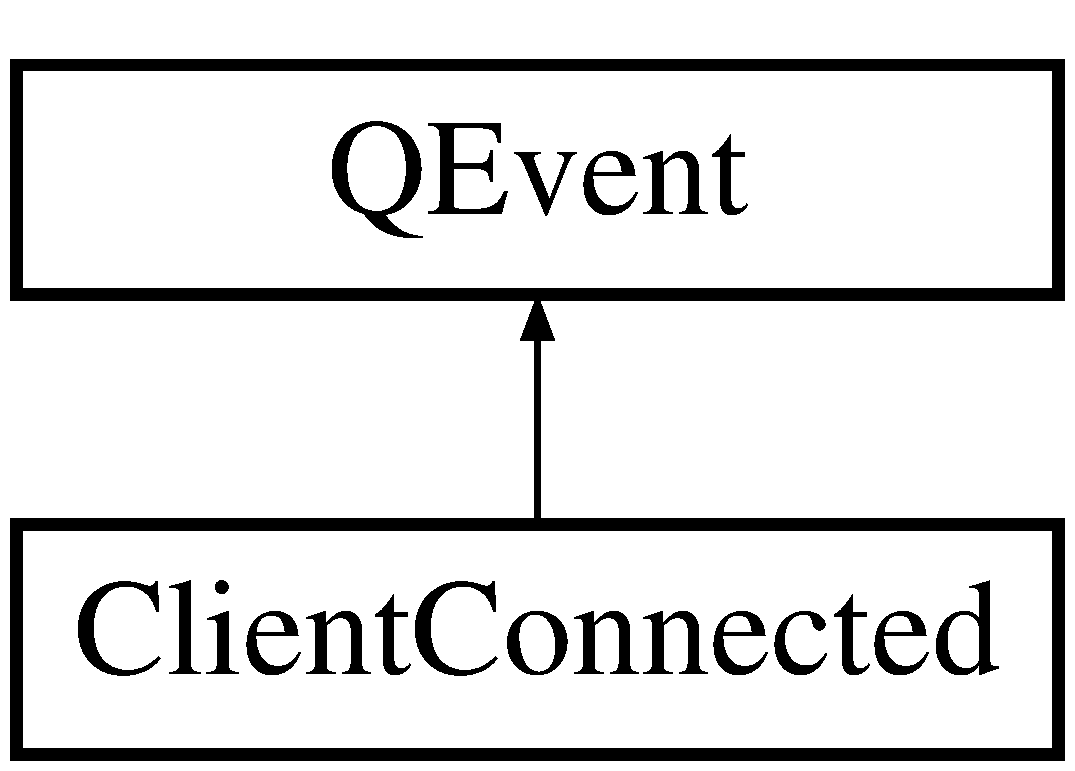
\includegraphics[height=2.000000cm]{class_client_connected}
\end{center}
\end{figure}


The documentation for this class was generated from the following file\+:\begin{DoxyCompactItemize}
\item 
Custom\+Events.\+h\end{DoxyCompactItemize}

\hypertarget{class_client_disconnected}{}\section{Client\+Disconnected Class Reference}
\label{class_client_disconnected}\index{Client\+Disconnected@{Client\+Disconnected}}
Inheritance diagram for Client\+Disconnected\+:\begin{figure}[H]
\begin{center}
\leavevmode
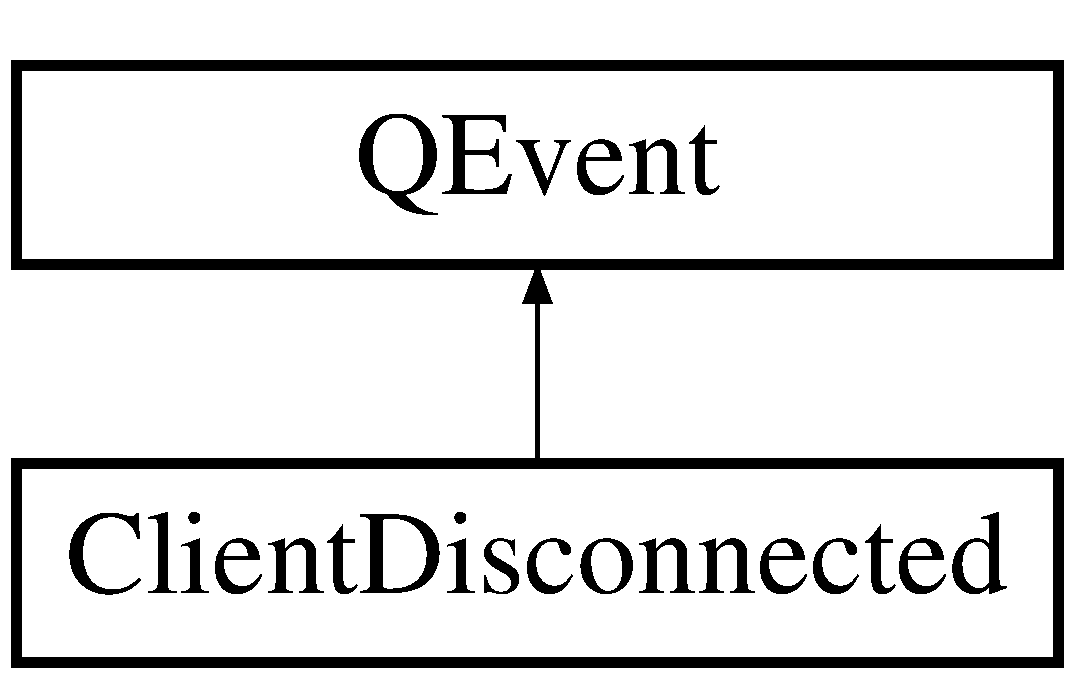
\includegraphics[height=2.000000cm]{class_client_disconnected}
\end{center}
\end{figure}


The documentation for this class was generated from the following file\+:\begin{DoxyCompactItemize}
\item 
Custom\+Events.\+h\end{DoxyCompactItemize}

\hypertarget{class_datagram_proccessed_received}{}\section{Datagram\+Proccessed\+Received Class Reference}
\label{class_datagram_proccessed_received}\index{Datagram\+Proccessed\+Received@{Datagram\+Proccessed\+Received}}
Inheritance diagram for Datagram\+Proccessed\+Received\+:\begin{figure}[H]
\begin{center}
\leavevmode
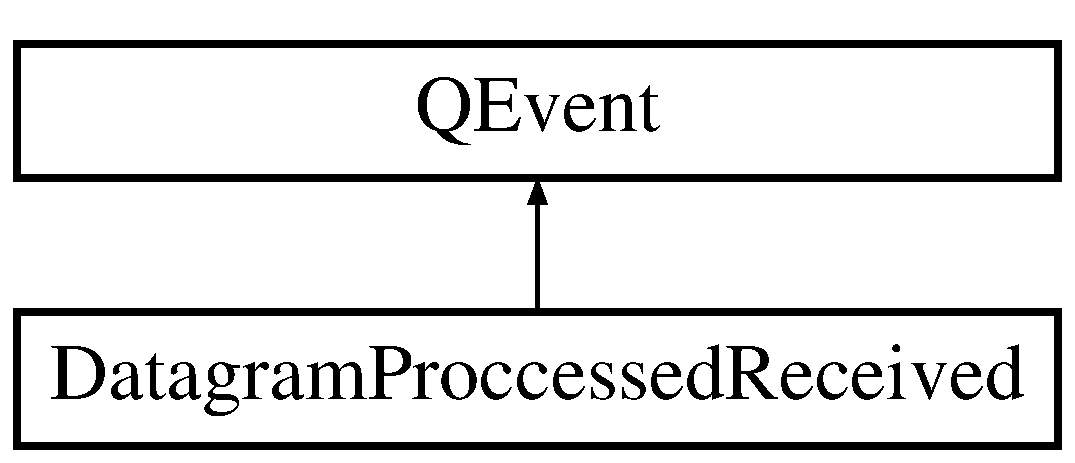
\includegraphics[height=2.000000cm]{class_datagram_proccessed_received}
\end{center}
\end{figure}


The documentation for this class was generated from the following file\+:\begin{DoxyCompactItemize}
\item 
Custom\+Events.\+h\end{DoxyCompactItemize}

\hypertarget{class_datagram_proccessed_sent}{}\section{Datagram\+Proccessed\+Sent Class Reference}
\label{class_datagram_proccessed_sent}\index{Datagram\+Proccessed\+Sent@{Datagram\+Proccessed\+Sent}}
Inheritance diagram for Datagram\+Proccessed\+Sent\+:\begin{figure}[H]
\begin{center}
\leavevmode
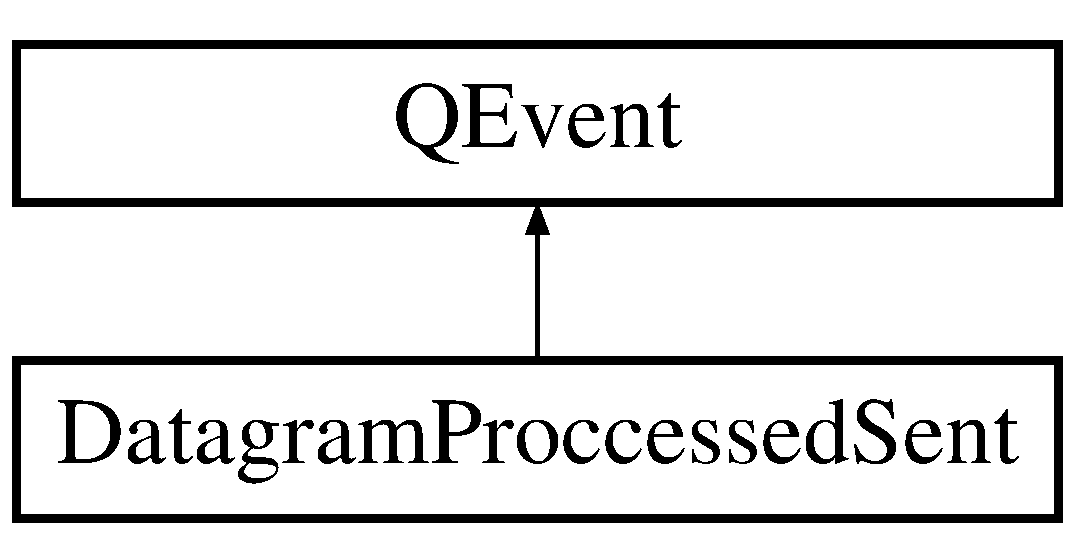
\includegraphics[height=2.000000cm]{class_datagram_proccessed_sent}
\end{center}
\end{figure}


The documentation for this class was generated from the following file\+:\begin{DoxyCompactItemize}
\item 
Custom\+Events.\+h\end{DoxyCompactItemize}

\hypertarget{struct_message}{}\section{Message Struct Reference}
\label{struct_message}\index{Message@{Message}}


Basic message class for the storing and sorting of messages.  




{\ttfamily \#include $<$message.\+h$>$}

\subsection*{Public Member Functions}
\begin{DoxyCompactItemize}
\item 
\hyperlink{struct_message_a4fc4f717b634e66070366cb7722d7761}{Message} ()
\item 
\hyperlink{struct_message_aa3f028e2b9674d7eb1712129deb01382}{Message} (Q\+Byte\+Array data, Q\+String message, Q\+Host\+Address senderip, quint16 senderinfo)
\end{DoxyCompactItemize}
\subsection*{Public Attributes}
\begin{DoxyCompactItemize}
\item 
\hypertarget{struct_message_a3ef7dc9dd3f7d356f48fe76fd97800a5}{}Q\+Byte\+Array {\bfseries data}\label{struct_message_a3ef7dc9dd3f7d356f48fe76fd97800a5}

\item 
\hypertarget{struct_message_aa1827946747d01ed5ef325cba3d86e1b}{}Q\+String {\bfseries message}\label{struct_message_aa1827946747d01ed5ef325cba3d86e1b}

\item 
\hypertarget{struct_message_a03891c75eb0cdc274337cb2e7ac11031}{}Q\+Host\+Address {\bfseries senderip}\label{struct_message_a03891c75eb0cdc274337cb2e7ac11031}

\item 
\hypertarget{struct_message_a38dbd0cc60b22aeed826ac30e9567da5}{}Q\+String {\bfseries senderip\+\_\+string}\label{struct_message_a38dbd0cc60b22aeed826ac30e9567da5}

\item 
\hypertarget{struct_message_ad1ada733d211a5270a164a1da128f6c0}{}quint16 {\bfseries senderinfo}\label{struct_message_ad1ada733d211a5270a164a1da128f6c0}

\item 
\hypertarget{struct_message_a049ad3d2cc26be505da1f4550805ec55}{}Q\+Time {\bfseries timestamp}\label{struct_message_a049ad3d2cc26be505da1f4550805ec55}

\item 
\hypertarget{struct_message_a037095a68df489f0da05ca6d3494d7d6}{}Q\+Date {\bfseries date}\label{struct_message_a037095a68df489f0da05ca6d3494d7d6}

\item 
\hypertarget{struct_message_a6fc78df47d3755e088e7c658db565fc5}{}Message\+Type {\bfseries type}\label{struct_message_a6fc78df47d3755e088e7c658db565fc5}

\end{DoxyCompactItemize}


\subsection{Detailed Description}
Basic message class for the storing and sorting of messages. 

When a datagram is received a message is constructed using the message, senderip the encrypted bytearray, and the sender I\+P and port.

The datetime is automatically set when a message is created and the type is set based on if the message contains a specific string. 

\subsection{Constructor \& Destructor Documentation}
\hypertarget{struct_message_a4fc4f717b634e66070366cb7722d7761}{}\index{Message@{Message}!Message@{Message}}
\index{Message@{Message}!Message@{Message}}
\subsubsection[{Message}]{\setlength{\rightskip}{0pt plus 5cm}Message\+::\+Message (
\begin{DoxyParamCaption}
{}
\end{DoxyParamCaption}
)}\label{struct_message_a4fc4f717b634e66070366cb7722d7761}
Constructor.

Constructs an Empty \hyperlink{struct_message}{Message} instance. \hypertarget{struct_message_aa3f028e2b9674d7eb1712129deb01382}{}\index{Message@{Message}!Message@{Message}}
\index{Message@{Message}!Message@{Message}}
\subsubsection[{Message}]{\setlength{\rightskip}{0pt plus 5cm}Message\+::\+Message (
\begin{DoxyParamCaption}
\item[{Q\+Byte\+Array}]{data, }
\item[{Q\+String}]{message, }
\item[{Q\+Host\+Address}]{senderip, }
\item[{quint16}]{senderinfo}
\end{DoxyParamCaption}
)\hspace{0.3cm}{\ttfamily [inline]}}\label{struct_message_aa3f028e2b9674d7eb1712129deb01382}
Constructor.

Constructs a \hyperlink{struct_message}{Message} instance using the given \begin{DoxyItemize}
\item . \end{DoxyItemize}


The documentation for this struct was generated from the following file\+:\begin{DoxyCompactItemize}
\item 
message.\+h\end{DoxyCompactItemize}

\hypertarget{class_message_handler}{}\section{Message\+Handler Class Reference}
\label{class_message_handler}\index{Message\+Handler@{Message\+Handler}}


Static messagehandler class for accessing the messages throughout the application.  




{\ttfamily \#include $<$messagehandler.\+h$>$}

Inheritance diagram for Message\+Handler\+:\begin{figure}[H]
\begin{center}
\leavevmode
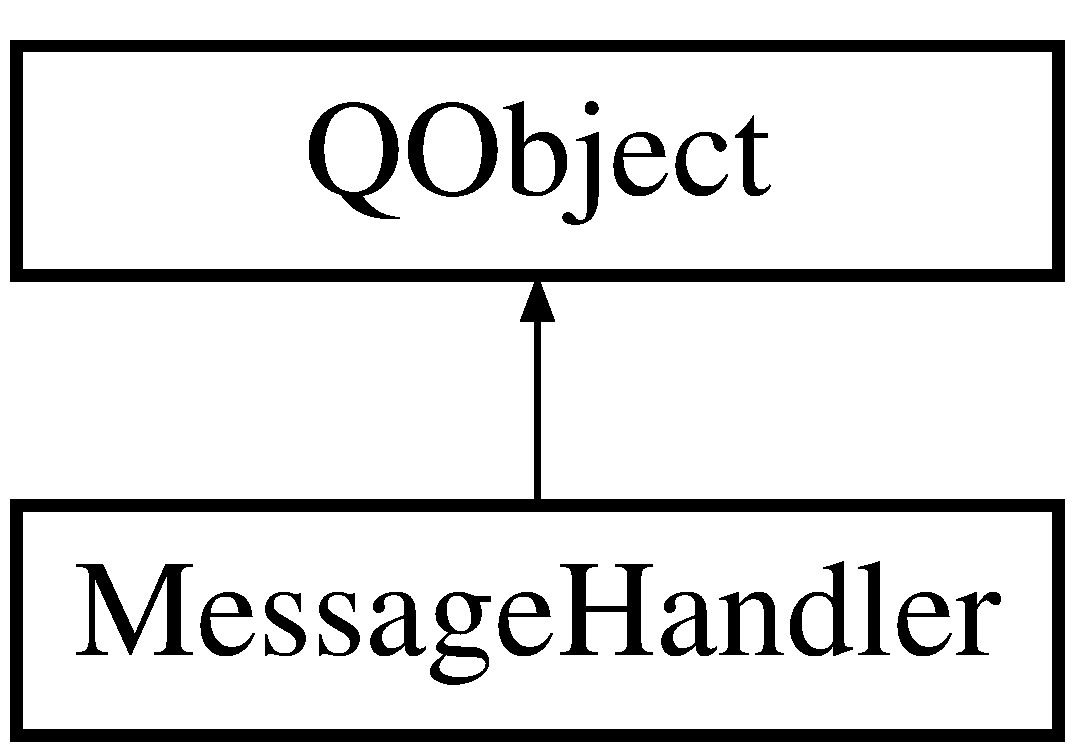
\includegraphics[height=2.000000cm]{class_message_handler}
\end{center}
\end{figure}
\subsection*{Public Member Functions}
\begin{DoxyCompactItemize}
\item 
\hyperlink{class_message_handler_a9dfaad39ced765947bf2dd27188de452}{Message\+Handler} (Q\+Object $\ast$parent=0)
\end{DoxyCompactItemize}
\subsection*{Static Public Member Functions}
\begin{DoxyCompactItemize}
\item 
static \hyperlink{struct_message}{Message} $\ast$ \hyperlink{class_message_handler_a42b14784fcc1502b639c656f9e2b2622}{get\+Most\+Recent\+Message} (bool received=true)
\item 
static void \hyperlink{class_message_handler_aa9e5166886e7e73e51f99ddf585249b1}{handle\+Message} (\hyperlink{struct_message}{Message} message, bool received)
\end{DoxyCompactItemize}
\subsection*{Static Private Attributes}
\begin{DoxyCompactItemize}
\item 
\hypertarget{class_message_handler_afab7e6704086a6098d5307ab62ee1035}{}static std\+::vector$<$ \hyperlink{struct_message}{Message} $>$ {\bfseries m\+\_\+sent\+Messages} = \{\}\label{class_message_handler_afab7e6704086a6098d5307ab62ee1035}

\item 
\hypertarget{class_message_handler_a32b68925a36229e748b8926b03c629c6}{}static std\+::vector$<$ \hyperlink{struct_message}{Message} $>$ {\bfseries m\+\_\+received\+Messages} = \{\}\label{class_message_handler_a32b68925a36229e748b8926b03c629c6}

\end{DoxyCompactItemize}


\subsection{Detailed Description}
Static messagehandler class for accessing the messages throughout the application. 

When a datagram is received a message object is created and then stored in a static vector, the vector is contained in this static \hyperlink{class_message_handler}{Message\+Handler} class so that they are accessable anywhere in the application. 

\subsection{Constructor \& Destructor Documentation}
\hypertarget{class_message_handler_a9dfaad39ced765947bf2dd27188de452}{}\index{Message\+Handler@{Message\+Handler}!Message\+Handler@{Message\+Handler}}
\index{Message\+Handler@{Message\+Handler}!Message\+Handler@{Message\+Handler}}
\subsubsection[{Message\+Handler}]{\setlength{\rightskip}{0pt plus 5cm}Message\+Handler\+::\+Message\+Handler (
\begin{DoxyParamCaption}
\item[{Q\+Object $\ast$}]{parent = {\ttfamily 0}}
\end{DoxyParamCaption}
)\hspace{0.3cm}{\ttfamily [explicit]}}\label{class_message_handler_a9dfaad39ced765947bf2dd27188de452}
Constructor.

This should never be called as \hyperlink{class_message_handler}{Message\+Handler} is a static class. 

\subsection{Member Function Documentation}
\hypertarget{class_message_handler_a42b14784fcc1502b639c656f9e2b2622}{}\index{Message\+Handler@{Message\+Handler}!get\+Most\+Recent\+Message@{get\+Most\+Recent\+Message}}
\index{get\+Most\+Recent\+Message@{get\+Most\+Recent\+Message}!Message\+Handler@{Message\+Handler}}
\subsubsection[{get\+Most\+Recent\+Message}]{\setlength{\rightskip}{0pt plus 5cm}{\bf Message} $\ast$ Message\+Handler\+::get\+Most\+Recent\+Message (
\begin{DoxyParamCaption}
\item[{bool}]{received = {\ttfamily true}}
\end{DoxyParamCaption}
)\hspace{0.3cm}{\ttfamily [static]}}\label{class_message_handler_a42b14784fcc1502b639c656f9e2b2622}
Returns a pointer to the most recent message received. \hypertarget{class_message_handler_aa9e5166886e7e73e51f99ddf585249b1}{}\index{Message\+Handler@{Message\+Handler}!handle\+Message@{handle\+Message}}
\index{handle\+Message@{handle\+Message}!Message\+Handler@{Message\+Handler}}
\subsubsection[{handle\+Message}]{\setlength{\rightskip}{0pt plus 5cm}void Message\+Handler\+::handle\+Message (
\begin{DoxyParamCaption}
\item[{{\bf Message}}]{message, }
\item[{bool}]{received}
\end{DoxyParamCaption}
)\hspace{0.3cm}{\ttfamily [static]}}\label{class_message_handler_aa9e5166886e7e73e51f99ddf585249b1}
Stores the given \begin{DoxyItemize}
\item in the static m\+\_\+sent\+Message or m\+\_\+received\+Message vector. \end{DoxyItemize}


The documentation for this class was generated from the following files\+:\begin{DoxyCompactItemize}
\item 
messagehandler.\+h\item 
messagehandler.\+cpp\end{DoxyCompactItemize}

\hypertarget{class_network_listener}{}\section{Network\+Listener Class Reference}
\label{class_network_listener}\index{Network\+Listener@{Network\+Listener}}


Network interface for sending and received datagrams.  




{\ttfamily \#include $<$networklistener.\+h$>$}

Inheritance diagram for Network\+Listener\+:\begin{figure}[H]
\begin{center}
\leavevmode
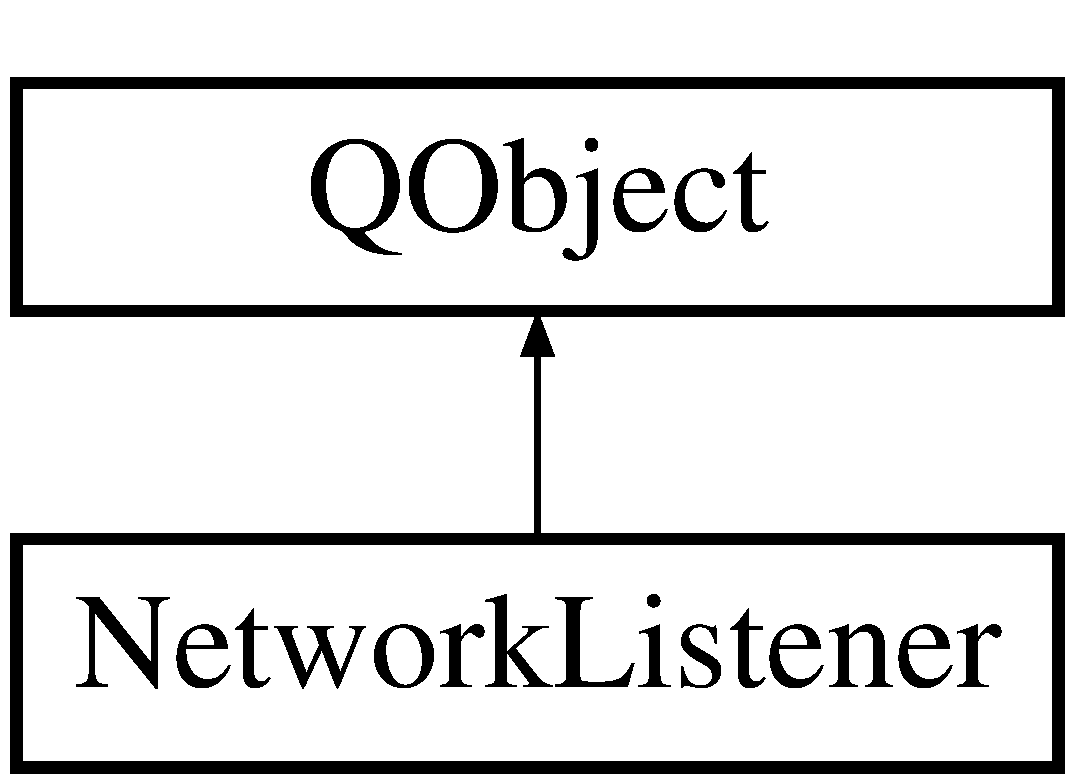
\includegraphics[height=2.000000cm]{class_network_listener}
\end{center}
\end{figure}
\subsection*{Public Slots}
\begin{DoxyCompactItemize}
\item 
void \hyperlink{class_network_listener_a831238cc68f68ecac14a9a5b3d330f1b}{process\+Pending\+Datagrams} ()
\item 
void \hyperlink{class_network_listener_a99aa1b32a4f64ad0c2d651b2a5ac9325}{send\+Datagram} (Q\+String a\+\_\+message, \hyperlink{struct_client}{Client} $\ast$a\+\_\+client=0)
\end{DoxyCompactItemize}
\subsection*{Public Member Functions}
\begin{DoxyCompactItemize}
\item 
\hyperlink{class_network_listener_ad0b176bc71290ed0d15705ee1ffdcf42}{Network\+Listener} (Q\+Object $\ast$parent=0)
\item 
\hyperlink{struct_client}{Client} $\ast$ \hyperlink{class_network_listener_a3bb629317b41d6b1f99a5b07b42a284f}{get\+Most\+Recent\+Client} ()
\item 
\hyperlink{struct_client}{Client} $\ast$ \hyperlink{class_network_listener_a9439e56b56ded28da4dc9c8584849e95}{get\+Most\+Recent\+Disconnected} ()
\item 
\hyperlink{struct_client}{Client} $\ast$ \hyperlink{class_network_listener_a30a1a0a5b42a426dc86ac131bd11aafd}{get\+Client} (Q\+String name)
\item 
void \hyperlink{class_network_listener_a989f81e745b1725562da7b6fcfadac83}{remove\+Client} (Q\+String name)
\item 
void \hyperlink{class_network_listener_aebdaf064bfc92c215266faa0a07ca61d}{send\+Hand\+Shake} (Q\+String name)
\item 
void \hyperlink{class_network_listener_a4905e63cbcdd10abd1cfdaff31364383}{send\+Hand\+Shake\+Reply} ()
\item 
void \hyperlink{class_network_listener_abd383f47c7878354e182093cd615ab23}{send\+Disconnect} (Q\+String name)
\end{DoxyCompactItemize}
\subsection*{Public Attributes}
\begin{DoxyCompactItemize}
\item 
\hypertarget{class_network_listener_af0f6d8c5a2b1b2c457e1e4ee68e1d4bf}{}Q\+String {\bfseries name}\label{class_network_listener_af0f6d8c5a2b1b2c457e1e4ee68e1d4bf}

\end{DoxyCompactItemize}
\subsection*{Private Attributes}
\begin{DoxyCompactItemize}
\item 
\hypertarget{class_network_listener_a4283b85857436ac617eeb4c93fdf11ac}{}Q\+Host\+Address {\bfseries group\+Address}\label{class_network_listener_a4283b85857436ac617eeb4c93fdf11ac}

\item 
\hypertarget{class_network_listener_a9941fd48019abc42514df6b204228b74}{}Q\+Host\+Address {\bfseries local\+Address}\label{class_network_listener_a9941fd48019abc42514df6b204228b74}

\item 
\hypertarget{class_network_listener_adaba275a4d4b8bd16506f13f95b1575a}{}Q\+Udp\+Socket $\ast$ {\bfseries udp\+Socket\+Out}\label{class_network_listener_adaba275a4d4b8bd16506f13f95b1575a}

\item 
\hypertarget{class_network_listener_a5209ce2c1fcde559cd7bb499582bc31c}{}Q\+Udp\+Socket $\ast$ {\bfseries udp\+Socket\+In}\label{class_network_listener_a5209ce2c1fcde559cd7bb499582bc31c}

\item 
\hypertarget{class_network_listener_ad9e784d4d6f035ecc02d4b47368e727f}{}std\+::vector$<$ \hyperlink{struct_client}{Client} $>$ {\bfseries m\+\_\+client\+List}\label{class_network_listener_ad9e784d4d6f035ecc02d4b47368e727f}

\item 
\hypertarget{class_network_listener_aa22cfac015aabb913b1e91410a57c7c8}{}std\+::vector$<$ \hyperlink{struct_client}{Client} $>$ {\bfseries m\+\_\+disconnected}\label{class_network_listener_aa22cfac015aabb913b1e91410a57c7c8}

\item 
\hypertarget{class_network_listener_adb41464b0923c725f94001b73e51a820}{}\hyperlink{class_simple_crypt}{Simple\+Crypt} {\bfseries cryptodevice}\label{class_network_listener_adb41464b0923c725f94001b73e51a820}

\end{DoxyCompactItemize}


\subsection{Detailed Description}
Network interface for sending and received datagrams. 

The \hyperlink{class_network_listener}{Network\+Listener} class has two udp\+Sockets, one that it listens for traffic and the other that it writes packets too. There is some basic loopback protection functionality so that packet sent by the host are not also received by the host.

This also handles the currently connected clients.

This class also controls the decryptions of datagrams. 

\subsection{Constructor \& Destructor Documentation}
\hypertarget{class_network_listener_ad0b176bc71290ed0d15705ee1ffdcf42}{}\index{Network\+Listener@{Network\+Listener}!Network\+Listener@{Network\+Listener}}
\index{Network\+Listener@{Network\+Listener}!Network\+Listener@{Network\+Listener}}
\subsubsection[{Network\+Listener}]{\setlength{\rightskip}{0pt plus 5cm}Network\+Listener\+::\+Network\+Listener (
\begin{DoxyParamCaption}
\item[{Q\+Object $\ast$}]{parent = {\ttfamily 0}}
\end{DoxyParamCaption}
)\hspace{0.3cm}{\ttfamily [explicit]}}\label{class_network_listener_ad0b176bc71290ed0d15705ee1ffdcf42}
Constructor.

Constructs a \hyperlink{class_network_listener}{Network\+Listener} instance. 

\subsection{Member Function Documentation}
\hypertarget{class_network_listener_a30a1a0a5b42a426dc86ac131bd11aafd}{}\index{Network\+Listener@{Network\+Listener}!get\+Client@{get\+Client}}
\index{get\+Client@{get\+Client}!Network\+Listener@{Network\+Listener}}
\subsubsection[{get\+Client}]{\setlength{\rightskip}{0pt plus 5cm}{\bf Client} $\ast$ Network\+Listener\+::get\+Client (
\begin{DoxyParamCaption}
\item[{Q\+String}]{name}
\end{DoxyParamCaption}
)}\label{class_network_listener_a30a1a0a5b42a426dc86ac131bd11aafd}
Returns a pointer to the client that matched the given \begin{DoxyItemize}
\item . \end{DoxyItemize}
\hypertarget{class_network_listener_a3bb629317b41d6b1f99a5b07b42a284f}{}\index{Network\+Listener@{Network\+Listener}!get\+Most\+Recent\+Client@{get\+Most\+Recent\+Client}}
\index{get\+Most\+Recent\+Client@{get\+Most\+Recent\+Client}!Network\+Listener@{Network\+Listener}}
\subsubsection[{get\+Most\+Recent\+Client}]{\setlength{\rightskip}{0pt plus 5cm}{\bf Client}$\ast$ Network\+Listener\+::get\+Most\+Recent\+Client (
\begin{DoxyParamCaption}
{}
\end{DoxyParamCaption}
)\hspace{0.3cm}{\ttfamily [inline]}}\label{class_network_listener_a3bb629317b41d6b1f99a5b07b42a284f}
Returns a pointer to the most recent client connected. \hypertarget{class_network_listener_a9439e56b56ded28da4dc9c8584849e95}{}\index{Network\+Listener@{Network\+Listener}!get\+Most\+Recent\+Disconnected@{get\+Most\+Recent\+Disconnected}}
\index{get\+Most\+Recent\+Disconnected@{get\+Most\+Recent\+Disconnected}!Network\+Listener@{Network\+Listener}}
\subsubsection[{get\+Most\+Recent\+Disconnected}]{\setlength{\rightskip}{0pt plus 5cm}{\bf Client}$\ast$ Network\+Listener\+::get\+Most\+Recent\+Disconnected (
\begin{DoxyParamCaption}
{}
\end{DoxyParamCaption}
)\hspace{0.3cm}{\ttfamily [inline]}}\label{class_network_listener_a9439e56b56ded28da4dc9c8584849e95}
Returns a pointer to the most recent client disconnected. \hypertarget{class_network_listener_a831238cc68f68ecac14a9a5b3d330f1b}{}\index{Network\+Listener@{Network\+Listener}!process\+Pending\+Datagrams@{process\+Pending\+Datagrams}}
\index{process\+Pending\+Datagrams@{process\+Pending\+Datagrams}!Network\+Listener@{Network\+Listener}}
\subsubsection[{process\+Pending\+Datagrams}]{\setlength{\rightskip}{0pt plus 5cm}void Network\+Listener\+::process\+Pending\+Datagrams (
\begin{DoxyParamCaption}
{}
\end{DoxyParamCaption}
)\hspace{0.3cm}{\ttfamily [slot]}}\label{class_network_listener_a831238cc68f68ecac14a9a5b3d330f1b}
Public slot function that is called when ready\+Read() on our udp\+Socket returns true.

Uses Q\+T's callback functionality to call a function when another function is called. \hypertarget{class_network_listener_a989f81e745b1725562da7b6fcfadac83}{}\index{Network\+Listener@{Network\+Listener}!remove\+Client@{remove\+Client}}
\index{remove\+Client@{remove\+Client}!Network\+Listener@{Network\+Listener}}
\subsubsection[{remove\+Client}]{\setlength{\rightskip}{0pt plus 5cm}void Network\+Listener\+::remove\+Client (
\begin{DoxyParamCaption}
\item[{Q\+String}]{name}
\end{DoxyParamCaption}
)}\label{class_network_listener_a989f81e745b1725562da7b6fcfadac83}
Removes the given \begin{DoxyItemize}
\item from the current client vector. \end{DoxyItemize}
\hypertarget{class_network_listener_a99aa1b32a4f64ad0c2d651b2a5ac9325}{}\index{Network\+Listener@{Network\+Listener}!send\+Datagram@{send\+Datagram}}
\index{send\+Datagram@{send\+Datagram}!Network\+Listener@{Network\+Listener}}
\subsubsection[{send\+Datagram}]{\setlength{\rightskip}{0pt plus 5cm}void Network\+Listener\+::send\+Datagram (
\begin{DoxyParamCaption}
\item[{Q\+String}]{a\+\_\+message, }
\item[{{\bf Client} $\ast$}]{a\+\_\+client = {\ttfamily 0}}
\end{DoxyParamCaption}
)\hspace{0.3cm}{\ttfamily [slot]}}\label{class_network_listener_a99aa1b32a4f64ad0c2d651b2a5ac9325}
Public slot function that is called when our submit button is clicked on the ui.

Send a datagram to the given client is the argument is specified otherwise it sends it to the entire multicast group.

Uses Q\+T's callback functionality to call a function when another function is called. \hypertarget{class_network_listener_abd383f47c7878354e182093cd615ab23}{}\index{Network\+Listener@{Network\+Listener}!send\+Disconnect@{send\+Disconnect}}
\index{send\+Disconnect@{send\+Disconnect}!Network\+Listener@{Network\+Listener}}
\subsubsection[{send\+Disconnect}]{\setlength{\rightskip}{0pt plus 5cm}void Network\+Listener\+::send\+Disconnect (
\begin{DoxyParamCaption}
\item[{Q\+String}]{name}
\end{DoxyParamCaption}
)}\label{class_network_listener_abd383f47c7878354e182093cd615ab23}
Send a disconnect packet using the given \begin{DoxyItemize}
\item as name. \end{DoxyItemize}
\hypertarget{class_network_listener_aebdaf064bfc92c215266faa0a07ca61d}{}\index{Network\+Listener@{Network\+Listener}!send\+Hand\+Shake@{send\+Hand\+Shake}}
\index{send\+Hand\+Shake@{send\+Hand\+Shake}!Network\+Listener@{Network\+Listener}}
\subsubsection[{send\+Hand\+Shake}]{\setlength{\rightskip}{0pt plus 5cm}void Network\+Listener\+::send\+Hand\+Shake (
\begin{DoxyParamCaption}
\item[{Q\+String}]{name}
\end{DoxyParamCaption}
)}\label{class_network_listener_aebdaf064bfc92c215266faa0a07ca61d}
Send a handshake packet using the given \begin{DoxyItemize}
\item as name. \end{DoxyItemize}
\hypertarget{class_network_listener_a4905e63cbcdd10abd1cfdaff31364383}{}\index{Network\+Listener@{Network\+Listener}!send\+Hand\+Shake\+Reply@{send\+Hand\+Shake\+Reply}}
\index{send\+Hand\+Shake\+Reply@{send\+Hand\+Shake\+Reply}!Network\+Listener@{Network\+Listener}}
\subsubsection[{send\+Hand\+Shake\+Reply}]{\setlength{\rightskip}{0pt plus 5cm}void Network\+Listener\+::send\+Hand\+Shake\+Reply (
\begin{DoxyParamCaption}
{}
\end{DoxyParamCaption}
)}\label{class_network_listener_a4905e63cbcdd10abd1cfdaff31364383}
Send a handshake reply packet. 

The documentation for this class was generated from the following files\+:\begin{DoxyCompactItemize}
\item 
networklistener.\+h\item 
networklistener.\+cpp\end{DoxyCompactItemize}

\hypertarget{class_simple_crypt}{}\section{Simple\+Crypt Class Reference}
\label{class_simple_crypt}\index{Simple\+Crypt@{Simple\+Crypt}}


Simple encryption and decryption of strings and byte arrays.  




{\ttfamily \#include $<$simplecrypt.\+h$>$}

\subsection*{Public Types}
\begin{DoxyCompactItemize}
\item 
enum \hyperlink{class_simple_crypt_a25298e746f175cf175a18f082092ca8e}{Compression\+Mode} \{ \hyperlink{class_simple_crypt_a25298e746f175cf175a18f082092ca8ea8d04b76ed73553456ec87e88b18ddc66}{Compression\+Auto}, 
\hyperlink{class_simple_crypt_a25298e746f175cf175a18f082092ca8ea10aec29129f4e6d08c4f61d7008ec8f7}{Compression\+Always}, 
\hyperlink{class_simple_crypt_a25298e746f175cf175a18f082092ca8eadc794d925e3af54dcef9a24ee3f60f6d}{Compression\+Never}
 \}
\item 
enum \hyperlink{class_simple_crypt_a42a5172e558d346b28421cc4e85feb2d}{Integrity\+Protection\+Mode} \{ \hyperlink{class_simple_crypt_a42a5172e558d346b28421cc4e85feb2da75547c41ccde1fb3d4db9f8c27164e4c}{Protection\+None}, 
\hyperlink{class_simple_crypt_a42a5172e558d346b28421cc4e85feb2dab6ccee9e9680f70c79213647c7814e5c}{Protection\+Checksum}, 
\hyperlink{class_simple_crypt_a42a5172e558d346b28421cc4e85feb2daf915c42837795744edbc5254eb93154f}{Protection\+Hash}
 \}
\item 
enum \hyperlink{class_simple_crypt_ab7f81049e78f021b55a36f7cfac5a09b}{Error} \{ \hyperlink{class_simple_crypt_ab7f81049e78f021b55a36f7cfac5a09ba77b7389ae8659e97df448c8fff79ca83}{Error\+No\+Error}, 
\hyperlink{class_simple_crypt_ab7f81049e78f021b55a36f7cfac5a09bacfb6271ef5415fe5e6a0e5ee3094f3a7}{Error\+No\+Key\+Set}, 
\hyperlink{class_simple_crypt_ab7f81049e78f021b55a36f7cfac5a09ba4c43644f04a0eefc3ed2205223f19479}{Error\+Unknown\+Version}, 
\hyperlink{class_simple_crypt_ab7f81049e78f021b55a36f7cfac5a09ba8566157b59e4662d0400b34249918e88}{Error\+Integrity\+Failed}
 \}
\item 
\hypertarget{class_simple_crypt_abc7918ae3afd91a98831fad119add27a}{}enum {\bfseries Crypto\+Flag} \{ {\bfseries Crypto\+Flag\+None} = 0, 
{\bfseries Crypto\+Flag\+Compression} = 0x01, 
{\bfseries Crypto\+Flag\+Checksum} = 0x02, 
{\bfseries Crypto\+Flag\+Hash} = 0x04
 \}\label{class_simple_crypt_abc7918ae3afd91a98831fad119add27a}

\end{DoxyCompactItemize}
\subsection*{Public Member Functions}
\begin{DoxyCompactItemize}
\item 
\hyperlink{class_simple_crypt_ac474d12cfa9f93bfecea35891831046d}{Simple\+Crypt} ()
\item 
\hyperlink{class_simple_crypt_a65942757b85b3dd36618ea3edc5ceb89}{Simple\+Crypt} (quint64 key)
\item 
void \hyperlink{class_simple_crypt_aa7aad9ed2e88b883ba9214c7d9928745}{set\+Key} (quint64 key)
\item 
void \hyperlink{class_simple_crypt_a7aa2679a2350622c649e8448545ae8a4}{gen\+Key} ()
\item 
\hypertarget{class_simple_crypt_aa7cab41b041f1fbe1c62e484fea895ce}{}bool \hyperlink{class_simple_crypt_aa7cab41b041f1fbe1c62e484fea895ce}{has\+Key} () const \label{class_simple_crypt_aa7cab41b041f1fbe1c62e484fea895ce}

\begin{DoxyCompactList}\small\item\em generates a key and then sets it -\/ based on a timestamp that will change every 24 hours each client that uses this will generate the same key for the 24 hour period \end{DoxyCompactList}\item 
void \hyperlink{class_simple_crypt_adc6c6355aa276c0d3516f7ad273f063b}{set\+Compression\+Mode} (\hyperlink{class_simple_crypt_a25298e746f175cf175a18f082092ca8e}{Compression\+Mode} mode)
\item 
\hyperlink{class_simple_crypt_a25298e746f175cf175a18f082092ca8e}{Compression\+Mode} \hyperlink{class_simple_crypt_a303253756b925678e53bafc8b72a4e96}{compression\+Mode} () const 
\item 
void \hyperlink{class_simple_crypt_a4fef5e6d3246ee57d6a7b68475b12b8b}{set\+Integrity\+Protection\+Mode} (\hyperlink{class_simple_crypt_a42a5172e558d346b28421cc4e85feb2d}{Integrity\+Protection\+Mode} mode)
\item 
\hyperlink{class_simple_crypt_a42a5172e558d346b28421cc4e85feb2d}{Integrity\+Protection\+Mode} \hyperlink{class_simple_crypt_a81929610d0fd5667db83603f396ddb66}{integrity\+Protection\+Mode} () const 
\item 
\hyperlink{class_simple_crypt_ab7f81049e78f021b55a36f7cfac5a09b}{Error} \hyperlink{class_simple_crypt_a123562e29377ab26e3b398b588f596d9}{last\+Error} () const 
\item 
Q\+String \hyperlink{class_simple_crypt_af26a3d3c6cef9732190c1d2c6a53a5b5}{encrypt\+To\+String} (const Q\+String \&plaintext)
\item 
Q\+String \hyperlink{class_simple_crypt_aa72b79bf7a5bb971bf3b0a52b9247efd}{encrypt\+To\+String} (Q\+Byte\+Array plaintext)
\item 
Q\+Byte\+Array \hyperlink{class_simple_crypt_ae1991c7748b2bb74468bee0be372d2c4}{encrypt\+To\+Byte\+Array} (const Q\+String \&plaintext)
\item 
Q\+Byte\+Array \hyperlink{class_simple_crypt_a741305d04e86bcb7d4625b05bf234887}{encrypt\+To\+Byte\+Array} (Q\+Byte\+Array plaintext)
\item 
Q\+String \hyperlink{class_simple_crypt_aa454cf372b534fd5ffaa2c5bd0fa57ea}{decrypt\+To\+String} (const Q\+String \&cyphertext)
\item 
Q\+Byte\+Array \hyperlink{class_simple_crypt_ad6785e087d449a1aa80c39248e98fcda}{decrypt\+To\+Byte\+Array} (const Q\+String \&cyphertext)
\item 
Q\+String \hyperlink{class_simple_crypt_ad1a3257cefee43773803ec1b12654f92}{decrypt\+To\+String} (Q\+Byte\+Array cypher)
\item 
Q\+Byte\+Array \hyperlink{class_simple_crypt_a4babb69e45849f672574a26b6433c85a}{decrypt\+To\+Byte\+Array} (Q\+Byte\+Array cypher)
\item 
\hypertarget{class_simple_crypt_a710fb3871372ccddd6450f73afca24eb}{}{\bfseries Q\+\_\+\+D\+E\+C\+L\+A\+R\+E\+\_\+\+F\+L\+A\+G\+S} (Crypto\+Flags, Crypto\+Flag)\label{class_simple_crypt_a710fb3871372ccddd6450f73afca24eb}

\end{DoxyCompactItemize}
\subsection*{Private Member Functions}
\begin{DoxyCompactItemize}
\item 
\hypertarget{class_simple_crypt_a0c315473b243f7a3f707a2d0fedf61b7}{}void {\bfseries split\+Key} ()\label{class_simple_crypt_a0c315473b243f7a3f707a2d0fedf61b7}

\end{DoxyCompactItemize}
\subsection*{Private Attributes}
\begin{DoxyCompactItemize}
\item 
\hypertarget{class_simple_crypt_aefc99e850635cde7f13fb58e73a338ab}{}quint64 {\bfseries m\+\_\+key}\label{class_simple_crypt_aefc99e850635cde7f13fb58e73a338ab}

\item 
\hypertarget{class_simple_crypt_aac0bcad9eef0d0488ece419ef32c25f9}{}Q\+Vector$<$ char $>$ {\bfseries m\+\_\+key\+Parts}\label{class_simple_crypt_aac0bcad9eef0d0488ece419ef32c25f9}

\item 
\hypertarget{class_simple_crypt_a6d9a5f9ee813f93a40226b27f84043d1}{}\hyperlink{class_simple_crypt_a25298e746f175cf175a18f082092ca8e}{Compression\+Mode} {\bfseries m\+\_\+compression\+Mode}\label{class_simple_crypt_a6d9a5f9ee813f93a40226b27f84043d1}

\item 
\hypertarget{class_simple_crypt_a0fe57e519baf899804281db986bb0f82}{}\hyperlink{class_simple_crypt_a42a5172e558d346b28421cc4e85feb2d}{Integrity\+Protection\+Mode} {\bfseries m\+\_\+protection\+Mode}\label{class_simple_crypt_a0fe57e519baf899804281db986bb0f82}

\item 
\hypertarget{class_simple_crypt_adccf15d36547ce4fe300e011774553ae}{}\hyperlink{class_simple_crypt_ab7f81049e78f021b55a36f7cfac5a09b}{Error} {\bfseries m\+\_\+last\+Error}\label{class_simple_crypt_adccf15d36547ce4fe300e011774553ae}

\end{DoxyCompactItemize}


\subsection{Detailed Description}
Simple encryption and decryption of strings and byte arrays. 

This class provides a simple implementation of encryption and decryption of strings and byte arrays.

The class uses a 64 bit key. Simply create an instance of the class, set the key, and use the \hyperlink{class_simple_crypt_af26a3d3c6cef9732190c1d2c6a53a5b5}{encrypt\+To\+String()} method to calculate an encrypted version of the input string. To decrypt that string again, use an instance of \hyperlink{class_simple_crypt}{Simple\+Crypt} initialized with the same key, and call the \hyperlink{class_simple_crypt_aa454cf372b534fd5ffaa2c5bd0fa57ea}{decrypt\+To\+String()} method with the encrypted string. If the key matches, the decrypted version of the string will be returned again.

If you do not provide a key, or if something else is wrong, the encryption and decryption function will return an empty string or will return a string containing nonsense. \hyperlink{class_simple_crypt_a123562e29377ab26e3b398b588f596d9}{last\+Error()} will return a value indicating if the method was succesful, and if not, why not.

\hyperlink{class_simple_crypt}{Simple\+Crypt} is prepared for the case that the encryption and decryption algorithm is changed in a later version, by prepending a version identifier to the cypertext. 

\subsection{Member Enumeration Documentation}
\hypertarget{class_simple_crypt_a25298e746f175cf175a18f082092ca8e}{}\index{Simple\+Crypt@{Simple\+Crypt}!Compression\+Mode@{Compression\+Mode}}
\index{Compression\+Mode@{Compression\+Mode}!Simple\+Crypt@{Simple\+Crypt}}
\subsubsection[{Compression\+Mode}]{\setlength{\rightskip}{0pt plus 5cm}enum {\bf Simple\+Crypt\+::\+Compression\+Mode}}\label{class_simple_crypt_a25298e746f175cf175a18f082092ca8e}
Compression\+Mode describes if compression will be applied to the data to be encrypted. \begin{Desc}
\item[Enumerator]\par
\begin{description}
\index{Compression\+Auto@{Compression\+Auto}!Simple\+Crypt@{Simple\+Crypt}}\index{Simple\+Crypt@{Simple\+Crypt}!Compression\+Auto@{Compression\+Auto}}\item[{\em 
\hypertarget{class_simple_crypt_a25298e746f175cf175a18f082092ca8ea8d04b76ed73553456ec87e88b18ddc66}{}Compression\+Auto\label{class_simple_crypt_a25298e746f175cf175a18f082092ca8ea8d04b76ed73553456ec87e88b18ddc66}
}]Only apply compression if that results in a shorter plaintext. \index{Compression\+Always@{Compression\+Always}!Simple\+Crypt@{Simple\+Crypt}}\index{Simple\+Crypt@{Simple\+Crypt}!Compression\+Always@{Compression\+Always}}\item[{\em 
\hypertarget{class_simple_crypt_a25298e746f175cf175a18f082092ca8ea10aec29129f4e6d08c4f61d7008ec8f7}{}Compression\+Always\label{class_simple_crypt_a25298e746f175cf175a18f082092ca8ea10aec29129f4e6d08c4f61d7008ec8f7}
}]Always apply compression. Note that for short inputs, a compression may result in longer data \index{Compression\+Never@{Compression\+Never}!Simple\+Crypt@{Simple\+Crypt}}\index{Simple\+Crypt@{Simple\+Crypt}!Compression\+Never@{Compression\+Never}}\item[{\em 
\hypertarget{class_simple_crypt_a25298e746f175cf175a18f082092ca8eadc794d925e3af54dcef9a24ee3f60f6d}{}Compression\+Never\label{class_simple_crypt_a25298e746f175cf175a18f082092ca8eadc794d925e3af54dcef9a24ee3f60f6d}
}]Never apply compression. \end{description}
\end{Desc}
\hypertarget{class_simple_crypt_ab7f81049e78f021b55a36f7cfac5a09b}{}\index{Simple\+Crypt@{Simple\+Crypt}!Error@{Error}}
\index{Error@{Error}!Simple\+Crypt@{Simple\+Crypt}}
\subsubsection[{Error}]{\setlength{\rightskip}{0pt plus 5cm}enum {\bf Simple\+Crypt\+::\+Error}}\label{class_simple_crypt_ab7f81049e78f021b55a36f7cfac5a09b}
Error describes the type of error that occured. \begin{Desc}
\item[Enumerator]\par
\begin{description}
\index{Error\+No\+Error@{Error\+No\+Error}!Simple\+Crypt@{Simple\+Crypt}}\index{Simple\+Crypt@{Simple\+Crypt}!Error\+No\+Error@{Error\+No\+Error}}\item[{\em 
\hypertarget{class_simple_crypt_ab7f81049e78f021b55a36f7cfac5a09ba77b7389ae8659e97df448c8fff79ca83}{}Error\+No\+Error\label{class_simple_crypt_ab7f81049e78f021b55a36f7cfac5a09ba77b7389ae8659e97df448c8fff79ca83}
}]No error occurred. \index{Error\+No\+Key\+Set@{Error\+No\+Key\+Set}!Simple\+Crypt@{Simple\+Crypt}}\index{Simple\+Crypt@{Simple\+Crypt}!Error\+No\+Key\+Set@{Error\+No\+Key\+Set}}\item[{\em 
\hypertarget{class_simple_crypt_ab7f81049e78f021b55a36f7cfac5a09bacfb6271ef5415fe5e6a0e5ee3094f3a7}{}Error\+No\+Key\+Set\label{class_simple_crypt_ab7f81049e78f021b55a36f7cfac5a09bacfb6271ef5415fe5e6a0e5ee3094f3a7}
}]No key was set. You can not encrypt or decrypt without a valid key. \index{Error\+Unknown\+Version@{Error\+Unknown\+Version}!Simple\+Crypt@{Simple\+Crypt}}\index{Simple\+Crypt@{Simple\+Crypt}!Error\+Unknown\+Version@{Error\+Unknown\+Version}}\item[{\em 
\hypertarget{class_simple_crypt_ab7f81049e78f021b55a36f7cfac5a09ba4c43644f04a0eefc3ed2205223f19479}{}Error\+Unknown\+Version\label{class_simple_crypt_ab7f81049e78f021b55a36f7cfac5a09ba4c43644f04a0eefc3ed2205223f19479}
}]The version of this data is unknown, or the data is otherwise not valid. \index{Error\+Integrity\+Failed@{Error\+Integrity\+Failed}!Simple\+Crypt@{Simple\+Crypt}}\index{Simple\+Crypt@{Simple\+Crypt}!Error\+Integrity\+Failed@{Error\+Integrity\+Failed}}\item[{\em 
\hypertarget{class_simple_crypt_ab7f81049e78f021b55a36f7cfac5a09ba8566157b59e4662d0400b34249918e88}{}Error\+Integrity\+Failed\label{class_simple_crypt_ab7f81049e78f021b55a36f7cfac5a09ba8566157b59e4662d0400b34249918e88}
}]The integrity check of the data failed. Perhaps the wrong key was used. \end{description}
\end{Desc}
\hypertarget{class_simple_crypt_a42a5172e558d346b28421cc4e85feb2d}{}\index{Simple\+Crypt@{Simple\+Crypt}!Integrity\+Protection\+Mode@{Integrity\+Protection\+Mode}}
\index{Integrity\+Protection\+Mode@{Integrity\+Protection\+Mode}!Simple\+Crypt@{Simple\+Crypt}}
\subsubsection[{Integrity\+Protection\+Mode}]{\setlength{\rightskip}{0pt plus 5cm}enum {\bf Simple\+Crypt\+::\+Integrity\+Protection\+Mode}}\label{class_simple_crypt_a42a5172e558d346b28421cc4e85feb2d}
Integrity\+Protection\+Mode describes measures taken to make it possible to detect problems with the data or wrong decryption keys.

Measures involve adding a checksum or a cryptograhpic hash to the data to be encrypted. This increases the length of the resulting cypertext, but makes it possible to check if the plaintext appears to be valid after decryption. \begin{Desc}
\item[Enumerator]\par
\begin{description}
\index{Protection\+None@{Protection\+None}!Simple\+Crypt@{Simple\+Crypt}}\index{Simple\+Crypt@{Simple\+Crypt}!Protection\+None@{Protection\+None}}\item[{\em 
\hypertarget{class_simple_crypt_a42a5172e558d346b28421cc4e85feb2da75547c41ccde1fb3d4db9f8c27164e4c}{}Protection\+None\label{class_simple_crypt_a42a5172e558d346b28421cc4e85feb2da75547c41ccde1fb3d4db9f8c27164e4c}
}]The integerity of the encrypted data is not protected. It is not really possible to detect a wrong key, for instance. \index{Protection\+Checksum@{Protection\+Checksum}!Simple\+Crypt@{Simple\+Crypt}}\index{Simple\+Crypt@{Simple\+Crypt}!Protection\+Checksum@{Protection\+Checksum}}\item[{\em 
\hypertarget{class_simple_crypt_a42a5172e558d346b28421cc4e85feb2dab6ccee9e9680f70c79213647c7814e5c}{}Protection\+Checksum\label{class_simple_crypt_a42a5172e558d346b28421cc4e85feb2dab6ccee9e9680f70c79213647c7814e5c}
}]A simple checksum is used to verify that the data is in order. If not, an empty string is returned. \index{Protection\+Hash@{Protection\+Hash}!Simple\+Crypt@{Simple\+Crypt}}\index{Simple\+Crypt@{Simple\+Crypt}!Protection\+Hash@{Protection\+Hash}}\item[{\em 
\hypertarget{class_simple_crypt_a42a5172e558d346b28421cc4e85feb2daf915c42837795744edbc5254eb93154f}{}Protection\+Hash\label{class_simple_crypt_a42a5172e558d346b28421cc4e85feb2daf915c42837795744edbc5254eb93154f}
}]A cryptographic hash is used to verify the integrity of the data. This method produces a much stronger, but longer check \end{description}
\end{Desc}


\subsection{Constructor \& Destructor Documentation}
\hypertarget{class_simple_crypt_ac474d12cfa9f93bfecea35891831046d}{}\index{Simple\+Crypt@{Simple\+Crypt}!Simple\+Crypt@{Simple\+Crypt}}
\index{Simple\+Crypt@{Simple\+Crypt}!Simple\+Crypt@{Simple\+Crypt}}
\subsubsection[{Simple\+Crypt}]{\setlength{\rightskip}{0pt plus 5cm}Simple\+Crypt\+::\+Simple\+Crypt (
\begin{DoxyParamCaption}
{}
\end{DoxyParamCaption}
)}\label{class_simple_crypt_ac474d12cfa9f93bfecea35891831046d}
Constructor.

Constructs a \hyperlink{class_simple_crypt}{Simple\+Crypt} instance without a valid key set on it. \hypertarget{class_simple_crypt_a65942757b85b3dd36618ea3edc5ceb89}{}\index{Simple\+Crypt@{Simple\+Crypt}!Simple\+Crypt@{Simple\+Crypt}}
\index{Simple\+Crypt@{Simple\+Crypt}!Simple\+Crypt@{Simple\+Crypt}}
\subsubsection[{Simple\+Crypt}]{\setlength{\rightskip}{0pt plus 5cm}Simple\+Crypt\+::\+Simple\+Crypt (
\begin{DoxyParamCaption}
\item[{quint64}]{key}
\end{DoxyParamCaption}
)\hspace{0.3cm}{\ttfamily [explicit]}}\label{class_simple_crypt_a65942757b85b3dd36618ea3edc5ceb89}
Constructor.

Constructs a \hyperlink{class_simple_crypt}{Simple\+Crypt} instance and initializes it with the given \begin{DoxyItemize}
\item key. \end{DoxyItemize}


\subsection{Member Function Documentation}
\hypertarget{class_simple_crypt_a303253756b925678e53bafc8b72a4e96}{}\index{Simple\+Crypt@{Simple\+Crypt}!compression\+Mode@{compression\+Mode}}
\index{compression\+Mode@{compression\+Mode}!Simple\+Crypt@{Simple\+Crypt}}
\subsubsection[{compression\+Mode}]{\setlength{\rightskip}{0pt plus 5cm}{\bf Compression\+Mode} Simple\+Crypt\+::compression\+Mode (
\begin{DoxyParamCaption}
{}
\end{DoxyParamCaption}
) const\hspace{0.3cm}{\ttfamily [inline]}}\label{class_simple_crypt_a303253756b925678e53bafc8b72a4e96}
Returns the Compression\+Mode that is currently in use. \hypertarget{class_simple_crypt_ad6785e087d449a1aa80c39248e98fcda}{}\index{Simple\+Crypt@{Simple\+Crypt}!decrypt\+To\+Byte\+Array@{decrypt\+To\+Byte\+Array}}
\index{decrypt\+To\+Byte\+Array@{decrypt\+To\+Byte\+Array}!Simple\+Crypt@{Simple\+Crypt}}
\subsubsection[{decrypt\+To\+Byte\+Array}]{\setlength{\rightskip}{0pt plus 5cm}Q\+Byte\+Array Simple\+Crypt\+::decrypt\+To\+Byte\+Array (
\begin{DoxyParamCaption}
\item[{const Q\+String \&}]{cyphertext}
\end{DoxyParamCaption}
)}\label{class_simple_crypt_ad6785e087d449a1aa80c39248e98fcda}
Decrypts a cyphertext string encrypted with this class with the set key back to the plain text version.

If an error occured, such as non-\/matching keys between encryption and decryption, an empty string or a string containing nonsense may be returned. \hypertarget{class_simple_crypt_a4babb69e45849f672574a26b6433c85a}{}\index{Simple\+Crypt@{Simple\+Crypt}!decrypt\+To\+Byte\+Array@{decrypt\+To\+Byte\+Array}}
\index{decrypt\+To\+Byte\+Array@{decrypt\+To\+Byte\+Array}!Simple\+Crypt@{Simple\+Crypt}}
\subsubsection[{decrypt\+To\+Byte\+Array}]{\setlength{\rightskip}{0pt plus 5cm}Q\+Byte\+Array Simple\+Crypt\+::decrypt\+To\+Byte\+Array (
\begin{DoxyParamCaption}
\item[{Q\+Byte\+Array}]{cypher}
\end{DoxyParamCaption}
)}\label{class_simple_crypt_a4babb69e45849f672574a26b6433c85a}
Decrypts a cyphertext binary encrypted with this class with the set key back to the plain text version.

If an error occured, such as non-\/matching keys between encryption and decryption, an empty string or a string containing nonsense may be returned. \hypertarget{class_simple_crypt_aa454cf372b534fd5ffaa2c5bd0fa57ea}{}\index{Simple\+Crypt@{Simple\+Crypt}!decrypt\+To\+String@{decrypt\+To\+String}}
\index{decrypt\+To\+String@{decrypt\+To\+String}!Simple\+Crypt@{Simple\+Crypt}}
\subsubsection[{decrypt\+To\+String}]{\setlength{\rightskip}{0pt plus 5cm}Q\+String Simple\+Crypt\+::decrypt\+To\+String (
\begin{DoxyParamCaption}
\item[{const Q\+String \&}]{cyphertext}
\end{DoxyParamCaption}
)}\label{class_simple_crypt_aa454cf372b534fd5ffaa2c5bd0fa57ea}
Decrypts a cyphertext string encrypted with this class with the set key back to the plain text version.

If an error occured, such as non-\/matching keys between encryption and decryption, an empty string or a string containing nonsense may be returned. \hypertarget{class_simple_crypt_ad1a3257cefee43773803ec1b12654f92}{}\index{Simple\+Crypt@{Simple\+Crypt}!decrypt\+To\+String@{decrypt\+To\+String}}
\index{decrypt\+To\+String@{decrypt\+To\+String}!Simple\+Crypt@{Simple\+Crypt}}
\subsubsection[{decrypt\+To\+String}]{\setlength{\rightskip}{0pt plus 5cm}Q\+String Simple\+Crypt\+::decrypt\+To\+String (
\begin{DoxyParamCaption}
\item[{Q\+Byte\+Array}]{cypher}
\end{DoxyParamCaption}
)}\label{class_simple_crypt_ad1a3257cefee43773803ec1b12654f92}
Decrypts a cyphertext binary encrypted with this class with the set key back to the plain text version.

If an error occured, such as non-\/matching keys between encryption and decryption, an empty string or a string containing nonsense may be returned. \hypertarget{class_simple_crypt_ae1991c7748b2bb74468bee0be372d2c4}{}\index{Simple\+Crypt@{Simple\+Crypt}!encrypt\+To\+Byte\+Array@{encrypt\+To\+Byte\+Array}}
\index{encrypt\+To\+Byte\+Array@{encrypt\+To\+Byte\+Array}!Simple\+Crypt@{Simple\+Crypt}}
\subsubsection[{encrypt\+To\+Byte\+Array}]{\setlength{\rightskip}{0pt plus 5cm}Q\+Byte\+Array Simple\+Crypt\+::encrypt\+To\+Byte\+Array (
\begin{DoxyParamCaption}
\item[{const Q\+String \&}]{plaintext}
\end{DoxyParamCaption}
)}\label{class_simple_crypt_ae1991c7748b2bb74468bee0be372d2c4}
Encrypts the \begin{DoxyItemize}
\item plaintext string with the key the class was initialized with, and returns a binary cyphertext in a Q\+Byte\+Array the result.\end{DoxyItemize}
This method returns a byte array, that is useable for storing a binary format. If you need a string you can store in a text file, use \hyperlink{class_simple_crypt_af26a3d3c6cef9732190c1d2c6a53a5b5}{encrypt\+To\+String()} instead. \hypertarget{class_simple_crypt_a741305d04e86bcb7d4625b05bf234887}{}\index{Simple\+Crypt@{Simple\+Crypt}!encrypt\+To\+Byte\+Array@{encrypt\+To\+Byte\+Array}}
\index{encrypt\+To\+Byte\+Array@{encrypt\+To\+Byte\+Array}!Simple\+Crypt@{Simple\+Crypt}}
\subsubsection[{encrypt\+To\+Byte\+Array}]{\setlength{\rightskip}{0pt plus 5cm}Q\+Byte\+Array Simple\+Crypt\+::encrypt\+To\+Byte\+Array (
\begin{DoxyParamCaption}
\item[{Q\+Byte\+Array}]{plaintext}
\end{DoxyParamCaption}
)}\label{class_simple_crypt_a741305d04e86bcb7d4625b05bf234887}
Encrypts the \begin{DoxyItemize}
\item plaintext Q\+Byte\+Array with the key the class was initialized with, and returns a binary cyphertext in a Q\+Byte\+Array the result.\end{DoxyItemize}
This method returns a byte array, that is useable for storing a binary format. If you need a string you can store in a text file, use \hyperlink{class_simple_crypt_af26a3d3c6cef9732190c1d2c6a53a5b5}{encrypt\+To\+String()} instead. \hypertarget{class_simple_crypt_af26a3d3c6cef9732190c1d2c6a53a5b5}{}\index{Simple\+Crypt@{Simple\+Crypt}!encrypt\+To\+String@{encrypt\+To\+String}}
\index{encrypt\+To\+String@{encrypt\+To\+String}!Simple\+Crypt@{Simple\+Crypt}}
\subsubsection[{encrypt\+To\+String}]{\setlength{\rightskip}{0pt plus 5cm}Q\+String Simple\+Crypt\+::encrypt\+To\+String (
\begin{DoxyParamCaption}
\item[{const Q\+String \&}]{plaintext}
\end{DoxyParamCaption}
)}\label{class_simple_crypt_af26a3d3c6cef9732190c1d2c6a53a5b5}
Encrypts the \begin{DoxyItemize}
\item plaintext string with the key the class was initialized with, and returns a cyphertext the result. The result is a base64 encoded version of the binary array that is the actual result of the string, so it can be stored easily in a text format. \end{DoxyItemize}
\hypertarget{class_simple_crypt_aa72b79bf7a5bb971bf3b0a52b9247efd}{}\index{Simple\+Crypt@{Simple\+Crypt}!encrypt\+To\+String@{encrypt\+To\+String}}
\index{encrypt\+To\+String@{encrypt\+To\+String}!Simple\+Crypt@{Simple\+Crypt}}
\subsubsection[{encrypt\+To\+String}]{\setlength{\rightskip}{0pt plus 5cm}Q\+String Simple\+Crypt\+::encrypt\+To\+String (
\begin{DoxyParamCaption}
\item[{Q\+Byte\+Array}]{plaintext}
\end{DoxyParamCaption}
)}\label{class_simple_crypt_aa72b79bf7a5bb971bf3b0a52b9247efd}
Encrypts the \begin{DoxyItemize}
\item plaintext Q\+Byte\+Array with the key the class was initialized with, and returns a cyphertext the result. The result is a base64 encoded version of the binary array that is the actual result of the encryption, so it can be stored easily in a text format. \end{DoxyItemize}
\hypertarget{class_simple_crypt_a7aa2679a2350622c649e8448545ae8a4}{}\index{Simple\+Crypt@{Simple\+Crypt}!gen\+Key@{gen\+Key}}
\index{gen\+Key@{gen\+Key}!Simple\+Crypt@{Simple\+Crypt}}
\subsubsection[{gen\+Key}]{\setlength{\rightskip}{0pt plus 5cm}void Simple\+Crypt\+::gen\+Key (
\begin{DoxyParamCaption}
{}
\end{DoxyParamCaption}
)}\label{class_simple_crypt_a7aa2679a2350622c649e8448545ae8a4}
Returns true if \hyperlink{class_simple_crypt}{Simple\+Crypt} has been initialized with a key. \hypertarget{class_simple_crypt_a81929610d0fd5667db83603f396ddb66}{}\index{Simple\+Crypt@{Simple\+Crypt}!integrity\+Protection\+Mode@{integrity\+Protection\+Mode}}
\index{integrity\+Protection\+Mode@{integrity\+Protection\+Mode}!Simple\+Crypt@{Simple\+Crypt}}
\subsubsection[{integrity\+Protection\+Mode}]{\setlength{\rightskip}{0pt plus 5cm}{\bf Integrity\+Protection\+Mode} Simple\+Crypt\+::integrity\+Protection\+Mode (
\begin{DoxyParamCaption}
{}
\end{DoxyParamCaption}
) const\hspace{0.3cm}{\ttfamily [inline]}}\label{class_simple_crypt_a81929610d0fd5667db83603f396ddb66}
Returns the Integrity\+Protection\+Mode that is currently in use. \hypertarget{class_simple_crypt_a123562e29377ab26e3b398b588f596d9}{}\index{Simple\+Crypt@{Simple\+Crypt}!last\+Error@{last\+Error}}
\index{last\+Error@{last\+Error}!Simple\+Crypt@{Simple\+Crypt}}
\subsubsection[{last\+Error}]{\setlength{\rightskip}{0pt plus 5cm}{\bf Error} Simple\+Crypt\+::last\+Error (
\begin{DoxyParamCaption}
{}
\end{DoxyParamCaption}
) const\hspace{0.3cm}{\ttfamily [inline]}}\label{class_simple_crypt_a123562e29377ab26e3b398b588f596d9}
Returns the last error that occurred. \hypertarget{class_simple_crypt_adc6c6355aa276c0d3516f7ad273f063b}{}\index{Simple\+Crypt@{Simple\+Crypt}!set\+Compression\+Mode@{set\+Compression\+Mode}}
\index{set\+Compression\+Mode@{set\+Compression\+Mode}!Simple\+Crypt@{Simple\+Crypt}}
\subsubsection[{set\+Compression\+Mode}]{\setlength{\rightskip}{0pt plus 5cm}void Simple\+Crypt\+::set\+Compression\+Mode (
\begin{DoxyParamCaption}
\item[{{\bf Compression\+Mode}}]{mode}
\end{DoxyParamCaption}
)\hspace{0.3cm}{\ttfamily [inline]}}\label{class_simple_crypt_adc6c6355aa276c0d3516f7ad273f063b}
Sets the compression mode to use when encrypting data. The default mode is Auto.

Note that decryption is not influenced by this mode, as the decryption recognizes what mode was used when encrypting. \hypertarget{class_simple_crypt_a4fef5e6d3246ee57d6a7b68475b12b8b}{}\index{Simple\+Crypt@{Simple\+Crypt}!set\+Integrity\+Protection\+Mode@{set\+Integrity\+Protection\+Mode}}
\index{set\+Integrity\+Protection\+Mode@{set\+Integrity\+Protection\+Mode}!Simple\+Crypt@{Simple\+Crypt}}
\subsubsection[{set\+Integrity\+Protection\+Mode}]{\setlength{\rightskip}{0pt plus 5cm}void Simple\+Crypt\+::set\+Integrity\+Protection\+Mode (
\begin{DoxyParamCaption}
\item[{{\bf Integrity\+Protection\+Mode}}]{mode}
\end{DoxyParamCaption}
)\hspace{0.3cm}{\ttfamily [inline]}}\label{class_simple_crypt_a4fef5e6d3246ee57d6a7b68475b12b8b}
Sets the integrity mode to use when encrypting data. The default mode is Checksum.

Note that decryption is not influenced by this mode, as the decryption recognizes what mode was used when encrypting. \hypertarget{class_simple_crypt_aa7aad9ed2e88b883ba9214c7d9928745}{}\index{Simple\+Crypt@{Simple\+Crypt}!set\+Key@{set\+Key}}
\index{set\+Key@{set\+Key}!Simple\+Crypt@{Simple\+Crypt}}
\subsubsection[{set\+Key}]{\setlength{\rightskip}{0pt plus 5cm}void Simple\+Crypt\+::set\+Key (
\begin{DoxyParamCaption}
\item[{quint64}]{key}
\end{DoxyParamCaption}
)}\label{class_simple_crypt_aa7aad9ed2e88b883ba9214c7d9928745}
(Re-\/) initializes the key with the given \begin{DoxyItemize}
\item key. \end{DoxyItemize}


The documentation for this class was generated from the following files\+:\begin{DoxyCompactItemize}
\item 
simplecrypt.\+h\item 
simplecrypt.\+cpp\end{DoxyCompactItemize}

\hypertarget{class_ui___window}{}\section{Ui\+\_\+\+Window Class Reference}
\label{class_ui___window}\index{Ui\+\_\+\+Window@{Ui\+\_\+\+Window}}
Inheritance diagram for Ui\+\_\+\+Window\+:\begin{figure}[H]
\begin{center}
\leavevmode
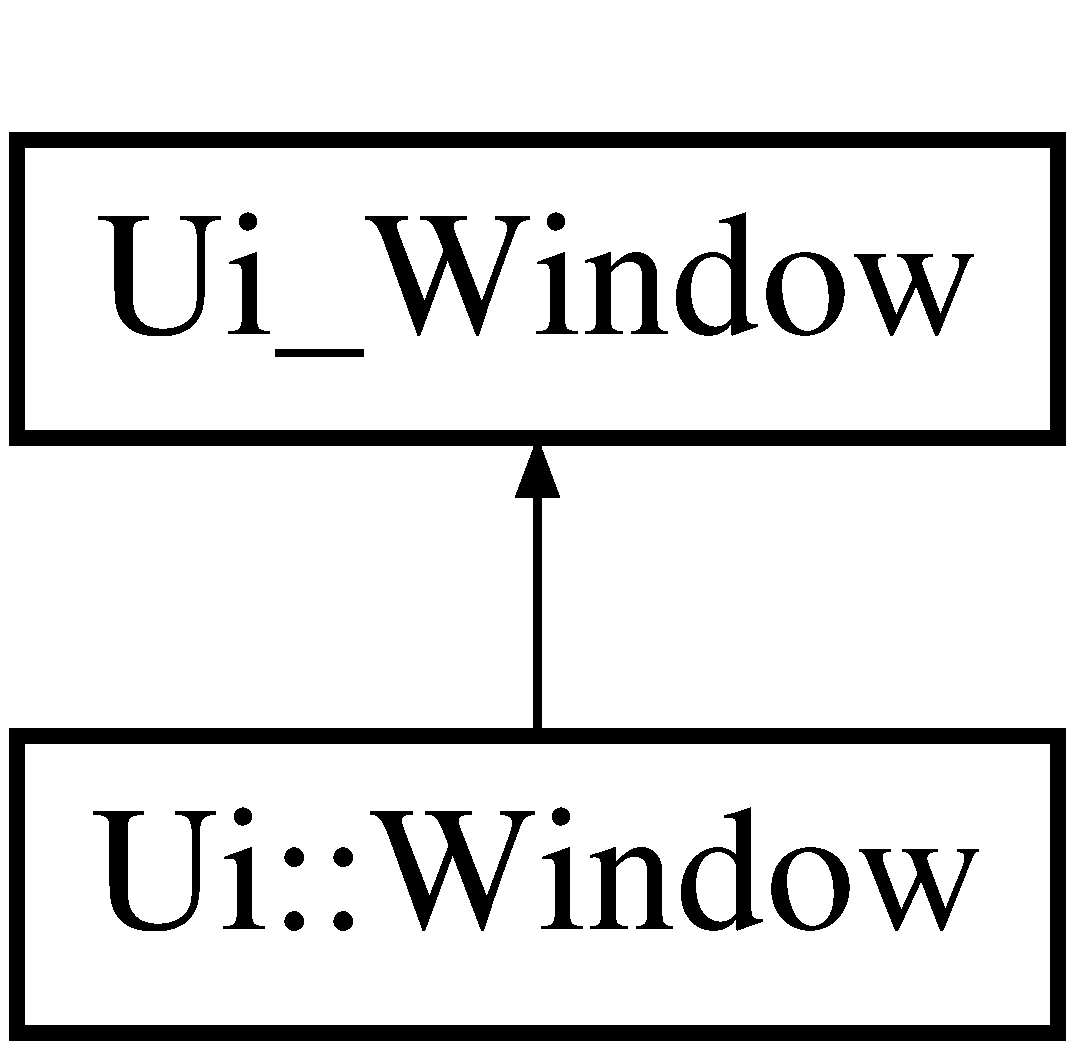
\includegraphics[height=2.000000cm]{class_ui___window}
\end{center}
\end{figure}
\subsection*{Public Member Functions}
\begin{DoxyCompactItemize}
\item 
\hypertarget{class_ui___window_a4b24c1d4c30a70b18fac50e906bacc79}{}void {\bfseries setup\+Ui} (Q\+Main\+Window $\ast$\hyperlink{class_window}{Window})\label{class_ui___window_a4b24c1d4c30a70b18fac50e906bacc79}

\item 
\hypertarget{class_ui___window_a40ce2989ba4cb35f824fa69735784d5c}{}void {\bfseries retranslate\+Ui} (Q\+Main\+Window $\ast$\hyperlink{class_window}{Window})\label{class_ui___window_a40ce2989ba4cb35f824fa69735784d5c}

\end{DoxyCompactItemize}
\subsection*{Public Attributes}
\begin{DoxyCompactItemize}
\item 
\hypertarget{class_ui___window_ace349d493eac0542f3185708568bb17c}{}Q\+Widget $\ast$ {\bfseries central\+Widget}\label{class_ui___window_ace349d493eac0542f3185708568bb17c}

\item 
\hypertarget{class_ui___window_aee8a875a7f0fe486efde941410ef45ad}{}Q\+Text\+Edit $\ast$ {\bfseries message\+Field}\label{class_ui___window_aee8a875a7f0fe486efde941410ef45ad}

\item 
\hypertarget{class_ui___window_a3857fc08f544f40007a582dd2e6e1157}{}Q\+Push\+Button $\ast$ {\bfseries clear\+Button}\label{class_ui___window_a3857fc08f544f40007a582dd2e6e1157}

\item 
\hypertarget{class_ui___window_af7fbdba2805a98d93247e73cad5facb0}{}Q\+Push\+Button $\ast$ {\bfseries submit\+Button}\label{class_ui___window_af7fbdba2805a98d93247e73cad5facb0}

\item 
\hypertarget{class_ui___window_a96095b2b170a45dddd9eeaab695a60f0}{}Q\+Label $\ast$ {\bfseries text\+Label}\label{class_ui___window_a96095b2b170a45dddd9eeaab695a60f0}

\item 
\hypertarget{class_ui___window_af7afa63d7866159c8b41b4251dacd245}{}Q\+Label $\ast$ {\bfseries text\+Label\+\_\+2}\label{class_ui___window_af7afa63d7866159c8b41b4251dacd245}

\item 
\hypertarget{class_ui___window_a96d01279964b6e2c30db8c29683f20f6}{}Q\+List\+Widget $\ast$ {\bfseries client\+List}\label{class_ui___window_a96d01279964b6e2c30db8c29683f20f6}

\item 
\hypertarget{class_ui___window_a7e6dc5f108787169ed4263658cffee06}{}Q\+Line\+Edit $\ast$ {\bfseries input\+Field}\label{class_ui___window_a7e6dc5f108787169ed4263658cffee06}

\item 
\hypertarget{class_ui___window_a94c557a0df03318a9bcaceb97fe9789c}{}Q\+Check\+Box $\ast$ {\bfseries check\+Box}\label{class_ui___window_a94c557a0df03318a9bcaceb97fe9789c}

\item 
\hypertarget{class_ui___window_ae1f82bcb6b78b1129ed4aa2da15fd080}{}Q\+Menu\+Bar $\ast$ {\bfseries menu\+Bar}\label{class_ui___window_ae1f82bcb6b78b1129ed4aa2da15fd080}

\item 
\hypertarget{class_ui___window_aa2ae6bf07615d6808fa4b6374d98ef01}{}Q\+Tool\+Bar $\ast$ {\bfseries main\+Tool\+Bar}\label{class_ui___window_aa2ae6bf07615d6808fa4b6374d98ef01}

\item 
\hypertarget{class_ui___window_ab6c076e3fb3fa6c143dfd85a13bee089}{}Q\+Status\+Bar $\ast$ {\bfseries status\+Bar}\label{class_ui___window_ab6c076e3fb3fa6c143dfd85a13bee089}

\end{DoxyCompactItemize}


The documentation for this class was generated from the following file\+:\begin{DoxyCompactItemize}
\item 
ui\+\_\+window.\+h\end{DoxyCompactItemize}

\hypertarget{class_window}{}\section{Window Class Reference}
\label{class_window}\index{Window@{Window}}


The Q\+Main\+Window class for our application, controls all ui and core application functionality.  




{\ttfamily \#include $<$window.\+h$>$}

Inheritance diagram for Window\+:\begin{figure}[H]
\begin{center}
\leavevmode
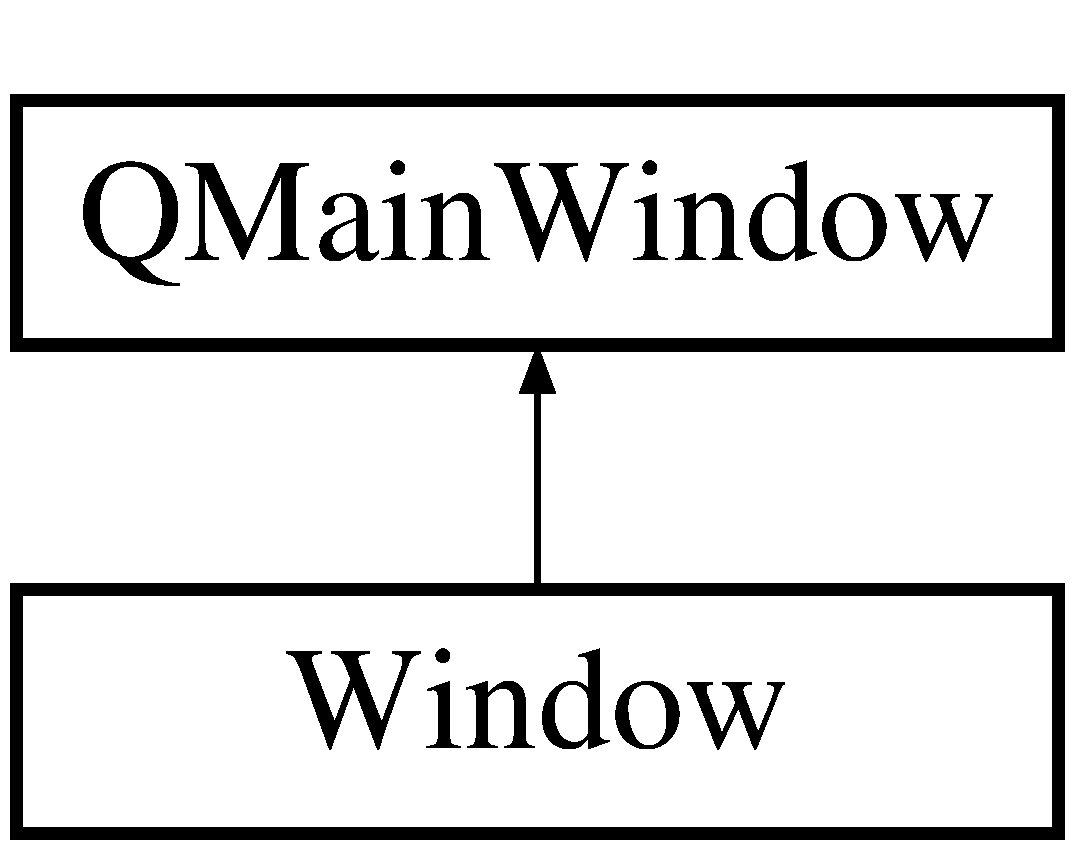
\includegraphics[height=2.000000cm]{class_window}
\end{center}
\end{figure}
\subsection*{Public Member Functions}
\begin{DoxyCompactItemize}
\item 
\hyperlink{class_window_ab27fe44e0834066236f79f244b02f67e}{Window} (Q\+Widget $\ast$parent=0)
\item 
bool \hyperlink{class_window_a0af393c895469fe202200eefb7e43e5e}{event} (Q\+Event $\ast$event)
\item 
void \hyperlink{class_window_a881940d1cff5b0ed7af7c601443e25d0}{set\+Name} (Q\+String pname)
\item 
const Q\+String \hyperlink{class_window_aa6c44398bab8bc643a1fe1472fe223e5}{get\+Name} ()
\item 
void \hyperlink{class_window_a9a63b5db3c68174e5cb50a4254f4dfe6}{play\+Alert} ()
\end{DoxyCompactItemize}
\subsection*{Private Slots}
\begin{DoxyCompactItemize}
\item 
void \hyperlink{class_window_a85e9aae377ed9b8179a162e2a286e7db}{send\+Message} ()
\item 
void \hyperlink{class_window_adfc7e2bf6ecd158d55025d05d8c45499}{toggle\+Important} ()
\item 
void \hyperlink{class_window_a1413affe9b805287af0c386d78346ea5}{open\+Help\+Doc} ()
\item 
void \hyperlink{class_window_abff605e7ff8389da3ee6704e396722d3}{save\+Message} (\hyperlink{struct_message}{Message} $\ast$message)
\item 
void \hyperlink{class_window_ac3c08dc3a42a66a69d105d5b8c96c28b}{update\+Current\+Client} (Q\+List\+Widget\+Item $\ast$item)
\end{DoxyCompactItemize}
\subsection*{Private Member Functions}
\begin{DoxyCompactItemize}
\item 
void \hyperlink{class_window_a45ee5a1dc49aa1847cc190fa99f618ae}{close\+Event} (Q\+Close\+Event $\ast$\hyperlink{class_window_a0af393c895469fe202200eefb7e43e5e}{event})
\item 
void \hyperlink{class_window_aa83b20409c3671cfc97c75a697565140}{tidy\+Messages} ()
\end{DoxyCompactItemize}
\subsection*{Private Attributes}
\begin{DoxyCompactItemize}
\item 
\hypertarget{class_window_a8f714eb54bfde4b16da703584ac08eea}{}\hyperlink{class_network_listener}{Network\+Listener} $\ast$ {\bfseries m\+\_\+network\+Listener}\label{class_window_a8f714eb54bfde4b16da703584ac08eea}

\item 
\hypertarget{class_window_a25e6c90561394c36b5012b2c8e74a72c}{}\hyperlink{class_ui_1_1_window}{Ui\+::\+Window} $\ast$ {\bfseries ui}\label{class_window_a25e6c90561394c36b5012b2c8e74a72c}

\item 
\hypertarget{class_window_ad717ad597f2a1277c0bd8fac55c74825}{}Q\+List\+Widget\+Item $\ast$ {\bfseries m\+\_\+current\+Client}\label{class_window_ad717ad597f2a1277c0bd8fac55c74825}

\item 
\hypertarget{class_window_a277444918604b04869aeb9bfebeceb16}{}Q\+String {\bfseries name}\label{class_window_a277444918604b04869aeb9bfebeceb16}

\item 
\hypertarget{class_window_a09f6515f36fa10c11773997ff933b5bf}{}Q\+Menu $\ast$ {\bfseries file\+Menu}\label{class_window_a09f6515f36fa10c11773997ff933b5bf}

\item 
\hypertarget{class_window_a0eec65ab015e4594d6821559d36a9b16}{}Q\+Menu $\ast$ {\bfseries edit\+Menu}\label{class_window_a0eec65ab015e4594d6821559d36a9b16}

\item 
\hypertarget{class_window_a6f609551d5591985f173c8c68505335a}{}Q\+Menu $\ast$ {\bfseries format\+Menu}\label{class_window_a6f609551d5591985f173c8c68505335a}

\item 
\hypertarget{class_window_a20e4c75cbfaf22452a06f95d34b9f882}{}Q\+Menu $\ast$ {\bfseries help\+Menu}\label{class_window_a20e4c75cbfaf22452a06f95d34b9f882}

\item 
\hypertarget{class_window_a9da0abf47d6c11e6671aae6d4b3c671e}{}Q\+Media\+Player $\ast$ {\bfseries player}\label{class_window_a9da0abf47d6c11e6671aae6d4b3c671e}

\item 
\hypertarget{class_window_a0b96a9e43c5b611359ed1d0c4ecea4bb}{}Q\+Regular\+Expression {\bfseries re}\label{class_window_a0b96a9e43c5b611359ed1d0c4ecea4bb}

\item 
\hypertarget{class_window_a6372feaa0a9d38275aa6a12bab5eeeab}{}Q\+Action $\ast$ {\bfseries save\+Act}\label{class_window_a6372feaa0a9d38275aa6a12bab5eeeab}

\item 
\hypertarget{class_window_ad333f8fa49cbbffacfbbf5737f160776}{}Q\+Action $\ast$ {\bfseries open\+Help}\label{class_window_ad333f8fa49cbbffacfbbf5737f160776}

\item 
\hypertarget{class_window_a61e25d1848a6dabe0ff43e85d3a93799}{}Q\+Action $\ast$ {\bfseries clear\+Act}\label{class_window_a61e25d1848a6dabe0ff43e85d3a93799}

\item 
\hypertarget{class_window_adf147b15222fd3eae05eae4fae2d0222}{}bool {\bfseries important} = false\label{class_window_adf147b15222fd3eae05eae4fae2d0222}

\end{DoxyCompactItemize}


\subsection{Detailed Description}
The Q\+Main\+Window class for our application, controls all ui and core application functionality. 

\hyperlink{class_window}{Window} controls all of our U\+I elements and provides the interface between the G\+U\+I and the underlying application functionality. 

\subsection{Constructor \& Destructor Documentation}
\hypertarget{class_window_ab27fe44e0834066236f79f244b02f67e}{}\index{Window@{Window}!Window@{Window}}
\index{Window@{Window}!Window@{Window}}
\subsubsection[{Window}]{\setlength{\rightskip}{0pt plus 5cm}Window\+::\+Window (
\begin{DoxyParamCaption}
\item[{Q\+Widget $\ast$}]{parent = {\ttfamily 0}}
\end{DoxyParamCaption}
)\hspace{0.3cm}{\ttfamily [explicit]}}\label{class_window_ab27fe44e0834066236f79f244b02f67e}
Constructor.

Constructs a \hyperlink{class_window}{Window} instance. 

\subsection{Member Function Documentation}
\hypertarget{class_window_a45ee5a1dc49aa1847cc190fa99f618ae}{}\index{Window@{Window}!close\+Event@{close\+Event}}
\index{close\+Event@{close\+Event}!Window@{Window}}
\subsubsection[{close\+Event}]{\setlength{\rightskip}{0pt plus 5cm}void Window\+::close\+Event (
\begin{DoxyParamCaption}
\item[{Q\+Close\+Event $\ast$}]{event}
\end{DoxyParamCaption}
)\hspace{0.3cm}{\ttfamily [private]}}\label{class_window_a45ee5a1dc49aa1847cc190fa99f618ae}
Override the Q\+Main\+Window \hyperlink{class_window_a45ee5a1dc49aa1847cc190fa99f618ae}{close\+Event()} function so we can handle our window close event to send our disconnect packet on window close. \hypertarget{class_window_a0af393c895469fe202200eefb7e43e5e}{}\index{Window@{Window}!event@{event}}
\index{event@{event}!Window@{Window}}
\subsubsection[{event}]{\setlength{\rightskip}{0pt plus 5cm}bool Window\+::event (
\begin{DoxyParamCaption}
\item[{Q\+Event $\ast$}]{event}
\end{DoxyParamCaption}
)}\label{class_window_a0af393c895469fe202200eefb7e43e5e}
Overrided the Q\+Main\+Window event function so that we can catch and handle our custom events. \hypertarget{class_window_aa6c44398bab8bc643a1fe1472fe223e5}{}\index{Window@{Window}!get\+Name@{get\+Name}}
\index{get\+Name@{get\+Name}!Window@{Window}}
\subsubsection[{get\+Name}]{\setlength{\rightskip}{0pt plus 5cm}const Q\+String Window\+::get\+Name (
\begin{DoxyParamCaption}
{}
\end{DoxyParamCaption}
)\hspace{0.3cm}{\ttfamily [inline]}}\label{class_window_aa6c44398bab8bc643a1fe1472fe223e5}
Returns our application name. \hypertarget{class_window_a1413affe9b805287af0c386d78346ea5}{}\index{Window@{Window}!open\+Help\+Doc@{open\+Help\+Doc}}
\index{open\+Help\+Doc@{open\+Help\+Doc}!Window@{Window}}
\subsubsection[{open\+Help\+Doc}]{\setlength{\rightskip}{0pt plus 5cm}void Window\+::open\+Help\+Doc (
\begin{DoxyParamCaption}
{}
\end{DoxyParamCaption}
)\hspace{0.3cm}{\ttfamily [private]}, {\ttfamily [slot]}}\label{class_window_a1413affe9b805287af0c386d78346ea5}
Public slot function that is called when filemenu help bar documentation option is pressed.

Toggles the help documentation generated by Doxygen.

Uses Q\+T's callback functionality to call a function when another function is called. \hypertarget{class_window_a9a63b5db3c68174e5cb50a4254f4dfe6}{}\index{Window@{Window}!play\+Alert@{play\+Alert}}
\index{play\+Alert@{play\+Alert}!Window@{Window}}
\subsubsection[{play\+Alert}]{\setlength{\rightskip}{0pt plus 5cm}void Window\+::play\+Alert (
\begin{DoxyParamCaption}
{}
\end{DoxyParamCaption}
)}\label{class_window_a9a63b5db3c68174e5cb50a4254f4dfe6}
Plays a short wav file, using for alerting when important messages have been received. \hypertarget{class_window_abff605e7ff8389da3ee6704e396722d3}{}\index{Window@{Window}!save\+Message@{save\+Message}}
\index{save\+Message@{save\+Message}!Window@{Window}}
\subsubsection[{save\+Message}]{\setlength{\rightskip}{0pt plus 5cm}void Window\+::save\+Message (
\begin{DoxyParamCaption}
\item[{{\bf Message} $\ast$}]{message}
\end{DoxyParamCaption}
)\hspace{0.3cm}{\ttfamily [private]}, {\ttfamily [slot]}}\label{class_window_abff605e7ff8389da3ee6704e396722d3}
Public slot function that is called when filemenu save bar save all option is pressed.

Currently unused.

Uses Q\+T's callback functionality to call a function when another function is called. \hypertarget{class_window_a85e9aae377ed9b8179a162e2a286e7db}{}\index{Window@{Window}!send\+Message@{send\+Message}}
\index{send\+Message@{send\+Message}!Window@{Window}}
\subsubsection[{send\+Message}]{\setlength{\rightskip}{0pt plus 5cm}void Window\+::send\+Message (
\begin{DoxyParamCaption}
{}
\end{DoxyParamCaption}
)\hspace{0.3cm}{\ttfamily [private]}, {\ttfamily [slot]}}\label{class_window_a85e9aae377ed9b8179a162e2a286e7db}
Public slot function that is called when ui submit button is clicked.

Uses Q\+T's callback functionality to call a function when another function is called. \hypertarget{class_window_a881940d1cff5b0ed7af7c601443e25d0}{}\index{Window@{Window}!set\+Name@{set\+Name}}
\index{set\+Name@{set\+Name}!Window@{Window}}
\subsubsection[{set\+Name}]{\setlength{\rightskip}{0pt plus 5cm}void Window\+::set\+Name (
\begin{DoxyParamCaption}
\item[{Q\+String}]{pname}
\end{DoxyParamCaption}
)\hspace{0.3cm}{\ttfamily [inline]}}\label{class_window_a881940d1cff5b0ed7af7c601443e25d0}
Sets our applcation name from the given \begin{DoxyItemize}
\item . \end{DoxyItemize}
\hypertarget{class_window_aa83b20409c3671cfc97c75a697565140}{}\index{Window@{Window}!tidy\+Messages@{tidy\+Messages}}
\index{tidy\+Messages@{tidy\+Messages}!Window@{Window}}
\subsubsection[{tidy\+Messages}]{\setlength{\rightskip}{0pt plus 5cm}void Window\+::tidy\+Messages (
\begin{DoxyParamCaption}
{}
\end{DoxyParamCaption}
)\hspace{0.3cm}{\ttfamily [private]}}\label{class_window_aa83b20409c3671cfc97c75a697565140}
Function used for tidying our message logs so that it does not contain messages older than 6 months. \hypertarget{class_window_adfc7e2bf6ecd158d55025d05d8c45499}{}\index{Window@{Window}!toggle\+Important@{toggle\+Important}}
\index{toggle\+Important@{toggle\+Important}!Window@{Window}}
\subsubsection[{toggle\+Important}]{\setlength{\rightskip}{0pt plus 5cm}void Window\+::toggle\+Important (
\begin{DoxyParamCaption}
{}
\end{DoxyParamCaption}
)\hspace{0.3cm}{\ttfamily [private]}, {\ttfamily [slot]}}\label{class_window_adfc7e2bf6ecd158d55025d05d8c45499}
Public slot function that is called when ui checkbox is clicked.

Uses Q\+T's callback functionality to call a function when another function is called. \hypertarget{class_window_ac3c08dc3a42a66a69d105d5b8c96c28b}{}\index{Window@{Window}!update\+Current\+Client@{update\+Current\+Client}}
\index{update\+Current\+Client@{update\+Current\+Client}!Window@{Window}}
\subsubsection[{update\+Current\+Client}]{\setlength{\rightskip}{0pt plus 5cm}void Window\+::update\+Current\+Client (
\begin{DoxyParamCaption}
\item[{Q\+List\+Widget\+Item $\ast$}]{item}
\end{DoxyParamCaption}
)\hspace{0.3cm}{\ttfamily [inline]}, {\ttfamily [private]}, {\ttfamily [slot]}}\label{class_window_ac3c08dc3a42a66a69d105d5b8c96c28b}
Public slot function that is called when a client is clicked in the client list.

Used for capurting our currently selected client for sending private messages.

Uses Q\+T's callback functionality to call a function when another function is called. 

The documentation for this class was generated from the following files\+:\begin{DoxyCompactItemize}
\item 
window.\+h\item 
window.\+cpp\end{DoxyCompactItemize}

\hypertarget{class_ui_1_1_window}{}\section{Ui\+:\+:Window Class Reference}
\label{class_ui_1_1_window}\index{Ui\+::\+Window@{Ui\+::\+Window}}
Inheritance diagram for Ui\+:\+:Window\+:\begin{figure}[H]
\begin{center}
\leavevmode
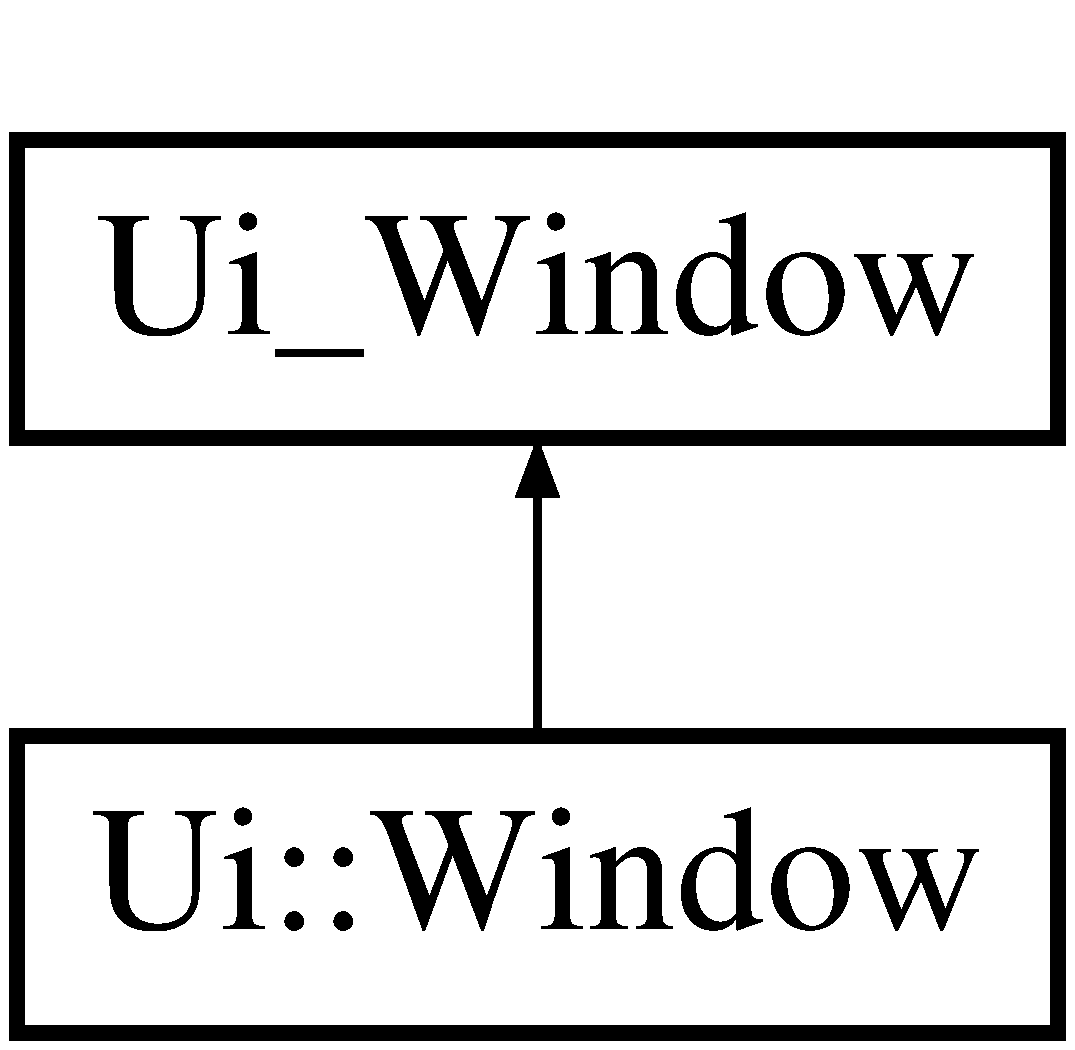
\includegraphics[height=2.000000cm]{class_ui_1_1_window}
\end{center}
\end{figure}
\subsection*{Additional Inherited Members}


The documentation for this class was generated from the following file\+:\begin{DoxyCompactItemize}
\item 
ui\+\_\+window.\+h\end{DoxyCompactItemize}

%--- End generated contents ---

% Index
\backmatter
\newpage
\phantomsection
\clearemptydoublepage
\addcontentsline{toc}{chapter}{Index}
\printindex

\end{document}
